\documentclass[twoside]{book}

% Packages required by doxygen
\usepackage{calc}
\usepackage{doxygen}
\usepackage{graphicx}
\usepackage[utf8]{inputenc}
\usepackage{makeidx}
\usepackage{multicol}
\usepackage{multirow}
\usepackage{textcomp}
\usepackage[table]{xcolor}

% Font selection
\usepackage[T1]{fontenc}
\usepackage{mathptmx}
\usepackage[scaled=.90]{helvet}
\usepackage{courier}
\usepackage{amssymb}
\usepackage{sectsty}
\renewcommand{\familydefault}{\sfdefault}
\allsectionsfont{%
  \fontseries{bc}\selectfont%
  \color{darkgray}%
}
\renewcommand{\DoxyLabelFont}{%
  \fontseries{bc}\selectfont%
  \color{darkgray}%
}

% Page & text layout
\usepackage{geometry}
\geometry{%
  a4paper,%
  top=2.5cm,%
  bottom=2.5cm,%
  left=2.5cm,%
  right=2.5cm%
}
\tolerance=750
\hfuzz=15pt
\hbadness=750
\setlength{\emergencystretch}{15pt}
\setlength{\parindent}{0cm}
\setlength{\parskip}{0.2cm}
\makeatletter
\renewcommand{\paragraph}{%
  \@startsection{paragraph}{4}{0ex}{-1.0ex}{1.0ex}{%
    \normalfont\normalsize\bfseries\SS@parafont%
  }%
}
\renewcommand{\subparagraph}{%
  \@startsection{subparagraph}{5}{0ex}{-1.0ex}{1.0ex}{%
    \normalfont\normalsize\bfseries\SS@subparafont%
  }%
}
\makeatother

% Headers & footers
\usepackage{fancyhdr}
\pagestyle{fancyplain}
\fancyhead[LE]{\fancyplain{}{\bfseries\thepage}}
\fancyhead[CE]{\fancyplain{}{}}
\fancyhead[RE]{\fancyplain{}{\bfseries\leftmark}}
\fancyhead[LO]{\fancyplain{}{\bfseries\rightmark}}
\fancyhead[CO]{\fancyplain{}{}}
\fancyhead[RO]{\fancyplain{}{\bfseries\thepage}}
\fancyfoot[LE]{\fancyplain{}{}}
\fancyfoot[CE]{\fancyplain{}{}}
\fancyfoot[RE]{\fancyplain{}{\bfseries\scriptsize Generated on Mon Oct 27 2014 12\-:35\-:55 for Ancle -\/ A\-C\-Slite N\-B\-I command line interface by Doxygen }}
\fancyfoot[LO]{\fancyplain{}{\bfseries\scriptsize Generated on Mon Oct 27 2014 12\-:35\-:55 for Ancle -\/ A\-C\-Slite N\-B\-I command line interface by Doxygen }}
\fancyfoot[CO]{\fancyplain{}{}}
\fancyfoot[RO]{\fancyplain{}{}}
\renewcommand{\footrulewidth}{0.4pt}
\renewcommand{\chaptermark}[1]{%
  \markboth{#1}{}%
}
\renewcommand{\sectionmark}[1]{%
  \markright{\thesection\ #1}%
}

% Indices & bibliography
\usepackage{natbib}
\usepackage[titles]{tocloft}
\setcounter{tocdepth}{3}
\setcounter{secnumdepth}{5}
\makeindex

% Hyperlinks (required, but should be loaded last)
\usepackage{ifpdf}
\ifpdf
  \usepackage[pdftex,pagebackref=true]{hyperref}
\else
  \usepackage[ps2pdf,pagebackref=true]{hyperref}
\fi
\hypersetup{%
  colorlinks=true,%
  linkcolor=blue,%
  citecolor=blue,%
  unicode%
}

% Custom commands
\newcommand{\clearemptydoublepage}{%
  \newpage{\pagestyle{empty}\cleardoublepage}%
}


%===== C O N T E N T S =====

\begin{document}

% Titlepage & ToC
\hypersetup{pageanchor=false}
\pagenumbering{roman}
\begin{titlepage}
\vspace*{7cm}
\begin{center}%
{\Large Ancle -\/ A\-C\-Slite N\-B\-I command line interface }\\
\vspace*{1cm}
{\large Generated by Doxygen 1.8.6}\\
\vspace*{0.5cm}
{\small Mon Oct 27 2014 12:35:55}\\
\end{center}
\end{titlepage}
\clearemptydoublepage
\tableofcontents
\clearemptydoublepage
\pagenumbering{arabic}
\hypersetup{pageanchor=true}

%--- Begin generated contents ---
\chapter{A\-N\-C\-L\-E main page}
\label{index}\hypertarget{index}{}Ancle -\/ A\-C\-S\-Light N\-B\-I Command Line interface \begin{DoxyAuthor}{Author}
Dario Protulipac 
\end{DoxyAuthor}
\begin{DoxyDate}{Date}
2014 
\end{DoxyDate}
\begin{DoxyCopyright}{Copyright}
G\-N\-U General Public License 
\end{DoxyCopyright}

\chapter{Data Structure Index}
\section{Data Structures}
Here are the data structures with brief descriptions\-:\begin{DoxyCompactList}
\item\contentsline{section}{\hyperlink{structacsdata}{acsdata} }{\pageref{structacsdata}}{}
\item\contentsline{section}{\hyperlink{structDeviceStruct}{Device\-Struct} }{\pageref{structDeviceStruct}}{}
\item\contentsline{section}{\hyperlink{structMemoryStruct}{Memory\-Struct} }{\pageref{structMemoryStruct}}{}
\end{DoxyCompactList}

\chapter{File Index}
\section{File List}
Here is a list of all files with brief descriptions\-:\begin{DoxyCompactList}
\item\contentsline{section}{src/\hyperlink{ancle_8c}{ancle.\-c} \\*Ancle -\/ A\-C\-S\-Light N\-B\-I Command Line interface main function }{\pageref{ancle_8c}}{}
\item\contentsline{section}{src/\hyperlink{ancle_8h}{ancle.\-h} \\*Main header file for A\-N\-C\-L\-E }{\pageref{ancle_8h}}{}
\item\contentsline{section}{src/\hyperlink{callcurl_8c}{callcurl.\-c} }{\pageref{callcurl_8c}}{}
\item\contentsline{section}{src/\hyperlink{config_8c}{config.\-c} }{\pageref{config_8c}}{}
\item\contentsline{section}{src/\hyperlink{getdevices_8c}{getdevices.\-c} \\*Hold basic actions for searching, registring and deleting devices }{\pageref{getdevices_8c}}{}
\item\contentsline{section}{src/\hyperlink{parseResponse_8c}{parse\-Response.\-c} \\*Functions for parsing responses from A\-C\-S server }{\pageref{parseResponse_8c}}{}
\item\contentsline{section}{src/\hyperlink{soapreq_8c}{soapreq.\-c} }{\pageref{soapreq_8c}}{}
\end{DoxyCompactList}

\chapter{Data Structure Documentation}
\hypertarget{structacsdata}{\section{acsdata Struct Reference}
\label{structacsdata}\index{acsdata@{acsdata}}
}


{\ttfamily \#include $<$ancle.\-h$>$}



Collaboration diagram for acsdata\-:\nopagebreak
\begin{figure}[H]
\begin{center}
\leavevmode
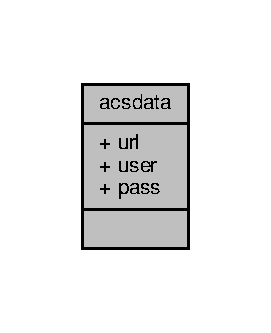
\includegraphics[width=130pt]{structacsdata__coll__graph}
\end{center}
\end{figure}
\subsection*{Data Fields}
\begin{DoxyCompactItemize}
\item 
char $\ast$ \hyperlink{structacsdata_a705fb13dc9a0271463e07f15ac785433}{url}
\item 
char $\ast$ \hyperlink{structacsdata_a5a023eb9d5cff7be3357abb6ebdd3172}{user}
\item 
char $\ast$ \hyperlink{structacsdata_aaaf4ce4a1ad46e1d3c8294001cd3caf3}{pass}
\end{DoxyCompactItemize}


\subsection{Detailed Description}
A\-C\-S server data 

Definition at line 76 of file ancle.\-h.



\subsection{Field Documentation}
\hypertarget{structacsdata_aaaf4ce4a1ad46e1d3c8294001cd3caf3}{\index{acsdata@{acsdata}!pass@{pass}}
\index{pass@{pass}!acsdata@{acsdata}}
\subsubsection[{pass}]{\setlength{\rightskip}{0pt plus 5cm}char$\ast$ acsdata\-::pass}}\label{structacsdata_aaaf4ce4a1ad46e1d3c8294001cd3caf3}


Definition at line 79 of file ancle.\-h.

\hypertarget{structacsdata_a705fb13dc9a0271463e07f15ac785433}{\index{acsdata@{acsdata}!url@{url}}
\index{url@{url}!acsdata@{acsdata}}
\subsubsection[{url}]{\setlength{\rightskip}{0pt plus 5cm}char$\ast$ acsdata\-::url}}\label{structacsdata_a705fb13dc9a0271463e07f15ac785433}


Definition at line 77 of file ancle.\-h.

\hypertarget{structacsdata_a5a023eb9d5cff7be3357abb6ebdd3172}{\index{acsdata@{acsdata}!user@{user}}
\index{user@{user}!acsdata@{acsdata}}
\subsubsection[{user}]{\setlength{\rightskip}{0pt plus 5cm}char$\ast$ acsdata\-::user}}\label{structacsdata_a5a023eb9d5cff7be3357abb6ebdd3172}


Definition at line 78 of file ancle.\-h.



The documentation for this struct was generated from the following file\-:\begin{DoxyCompactItemize}
\item 
src/\hyperlink{ancle_8h}{ancle.\-h}\end{DoxyCompactItemize}

\hypertarget{structDeviceStruct}{\section{Device\-Struct Struct Reference}
\label{structDeviceStruct}\index{Device\-Struct@{Device\-Struct}}
}


{\ttfamily \#include $<$ancle.\-h$>$}



Collaboration diagram for Device\-Struct\-:\nopagebreak
\begin{figure}[H]
\begin{center}
\leavevmode
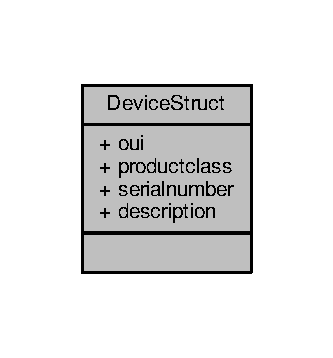
\includegraphics[width=160pt]{structDeviceStruct__coll__graph}
\end{center}
\end{figure}
\subsection*{Data Fields}
\begin{DoxyCompactItemize}
\item 
char $\ast$ \hyperlink{structDeviceStruct_ae8bec302b6b5c6d0a0fe1e64e4a45a37}{oui}
\item 
char $\ast$ \hyperlink{structDeviceStruct_a8411736ff451abaad5414e3dca6e671b}{productclass}
\item 
char $\ast$ \hyperlink{structDeviceStruct_a3d613c2cae19aac655b22ca3958ba601}{serialnumber}
\item 
char $\ast$ \hyperlink{structDeviceStruct_a7c6bdc123c89125b52aa347b0ef0d436}{description}
\end{DoxyCompactItemize}


\subsection{Detailed Description}
Basic device structure

Maximum string size (without null) is 64 bytes for every member of the structure exept oui which is 6 

Definition at line 61 of file ancle.\-h.



\subsection{Field Documentation}
\hypertarget{structDeviceStruct_a7c6bdc123c89125b52aa347b0ef0d436}{\index{Device\-Struct@{Device\-Struct}!description@{description}}
\index{description@{description}!DeviceStruct@{Device\-Struct}}
\subsubsection[{description}]{\setlength{\rightskip}{0pt plus 5cm}char$\ast$ Device\-Struct\-::description}}\label{structDeviceStruct_a7c6bdc123c89125b52aa347b0ef0d436}


Definition at line 65 of file ancle.\-h.

\hypertarget{structDeviceStruct_ae8bec302b6b5c6d0a0fe1e64e4a45a37}{\index{Device\-Struct@{Device\-Struct}!oui@{oui}}
\index{oui@{oui}!DeviceStruct@{Device\-Struct}}
\subsubsection[{oui}]{\setlength{\rightskip}{0pt plus 5cm}char$\ast$ Device\-Struct\-::oui}}\label{structDeviceStruct_ae8bec302b6b5c6d0a0fe1e64e4a45a37}


Definition at line 62 of file ancle.\-h.

\hypertarget{structDeviceStruct_a8411736ff451abaad5414e3dca6e671b}{\index{Device\-Struct@{Device\-Struct}!productclass@{productclass}}
\index{productclass@{productclass}!DeviceStruct@{Device\-Struct}}
\subsubsection[{productclass}]{\setlength{\rightskip}{0pt plus 5cm}char$\ast$ Device\-Struct\-::productclass}}\label{structDeviceStruct_a8411736ff451abaad5414e3dca6e671b}


Definition at line 63 of file ancle.\-h.

\hypertarget{structDeviceStruct_a3d613c2cae19aac655b22ca3958ba601}{\index{Device\-Struct@{Device\-Struct}!serialnumber@{serialnumber}}
\index{serialnumber@{serialnumber}!DeviceStruct@{Device\-Struct}}
\subsubsection[{serialnumber}]{\setlength{\rightskip}{0pt plus 5cm}char$\ast$ Device\-Struct\-::serialnumber}}\label{structDeviceStruct_a3d613c2cae19aac655b22ca3958ba601}


Definition at line 64 of file ancle.\-h.



The documentation for this struct was generated from the following file\-:\begin{DoxyCompactItemize}
\item 
src/\hyperlink{ancle_8h}{ancle.\-h}\end{DoxyCompactItemize}

\hypertarget{structMemoryStruct}{\section{Memory\-Struct Struct Reference}
\label{structMemoryStruct}\index{Memory\-Struct@{Memory\-Struct}}
}


{\ttfamily \#include $<$ancle.\-h$>$}



Collaboration diagram for Memory\-Struct\-:\nopagebreak
\begin{figure}[H]
\begin{center}
\leavevmode
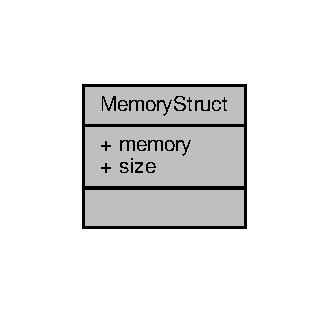
\includegraphics[width=158pt]{structMemoryStruct__coll__graph}
\end{center}
\end{figure}
\subsection*{Data Fields}
\begin{DoxyCompactItemize}
\item 
char $\ast$ \hyperlink{structMemoryStruct_a218a6fde0f367d44400542cbe523e943}{memory}
\item 
size\-\_\-t \hyperlink{structMemoryStruct_a79d6a7ad34b172f766c19d0846688440}{size}
\end{DoxyCompactItemize}


\subsection{Detailed Description}
Storage for retreived S\-O\-A\-P request 

Definition at line 49 of file ancle.\-h.



\subsection{Field Documentation}
\hypertarget{structMemoryStruct_a218a6fde0f367d44400542cbe523e943}{\index{Memory\-Struct@{Memory\-Struct}!memory@{memory}}
\index{memory@{memory}!MemoryStruct@{Memory\-Struct}}
\subsubsection[{memory}]{\setlength{\rightskip}{0pt plus 5cm}char$\ast$ Memory\-Struct\-::memory}}\label{structMemoryStruct_a218a6fde0f367d44400542cbe523e943}


Definition at line 50 of file ancle.\-h.

\hypertarget{structMemoryStruct_a79d6a7ad34b172f766c19d0846688440}{\index{Memory\-Struct@{Memory\-Struct}!size@{size}}
\index{size@{size}!MemoryStruct@{Memory\-Struct}}
\subsubsection[{size}]{\setlength{\rightskip}{0pt plus 5cm}size\-\_\-t Memory\-Struct\-::size}}\label{structMemoryStruct_a79d6a7ad34b172f766c19d0846688440}


Definition at line 51 of file ancle.\-h.



The documentation for this struct was generated from the following file\-:\begin{DoxyCompactItemize}
\item 
src/\hyperlink{ancle_8h}{ancle.\-h}\end{DoxyCompactItemize}

\chapter{File Documentation}
\hypertarget{ancle_8c}{\section{src/ancle.c File Reference}
\label{ancle_8c}\index{src/ancle.\-c@{src/ancle.\-c}}
}


Ancle -\/ A\-C\-S\-Light N\-B\-I Command Line interface main function.  


{\ttfamily \#include \char`\"{}config.\-h\char`\"{}}\\*
{\ttfamily \#include $<$ctype.\-h$>$}\\*
{\ttfamily \#include $<$stdio.\-h$>$}\\*
{\ttfamily \#include $<$stdlib.\-h$>$}\\*
{\ttfamily \#include $<$getopt.\-h$>$}\\*
{\ttfamily \#include \char`\"{}ancle.\-h\char`\"{}}\\*
Include dependency graph for ancle.\-c\-:\nopagebreak
\begin{figure}[H]
\begin{center}
\leavevmode
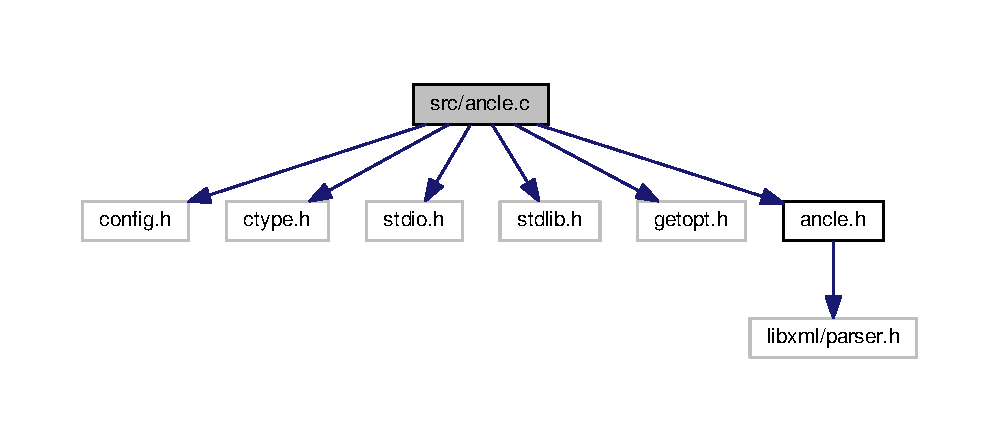
\includegraphics[width=350pt]{ancle_8c__incl}
\end{center}
\end{figure}
\subsection*{Functions}
\begin{DoxyCompactItemize}
\item 
void \hyperlink{ancle_8c_a853216ac51aa181669ff4d3de74058a7}{print\-\_\-help} ()
\item 
int \hyperlink{ancle_8c_a3c04138a5bfe5d72780bb7e82a18e627}{main} (int argc, char $\ast$$\ast$argv)
\end{DoxyCompactItemize}
\subsection*{Variables}
\begin{DoxyCompactItemize}
\item 
int \hyperlink{ancle_8c_a0b2caeb4b6f130be43e5a2f0267dd453}{verbose} = 0
\item 
int \hyperlink{ancle_8c_a7716c14cb5f92e9c141cdec3b980fa70}{yes} = 0
\end{DoxyCompactItemize}


\subsection{Detailed Description}
Ancle -\/ A\-C\-S\-Light N\-B\-I Command Line interface main function. This file contain main class will only take command line input paramteres and run function to parse configuration file. 

Definition in file \hyperlink{ancle_8c_source}{ancle.\-c}.



\subsection{Function Documentation}
\hypertarget{ancle_8c_a3c04138a5bfe5d72780bb7e82a18e627}{\index{ancle.\-c@{ancle.\-c}!main@{main}}
\index{main@{main}!ancle.c@{ancle.\-c}}
\subsubsection[{main}]{\setlength{\rightskip}{0pt plus 5cm}int main (
\begin{DoxyParamCaption}
\item[{int}]{argc, }
\item[{char $\ast$$\ast$}]{argv}
\end{DoxyParamCaption}
)}}\label{ancle_8c_a3c04138a5bfe5d72780bb7e82a18e627}
Just to get default input parameters and fire up required action for devices 

Definition at line 87 of file ancle.\-c.



Here is the call graph for this function\-:\nopagebreak
\begin{figure}[H]
\begin{center}
\leavevmode
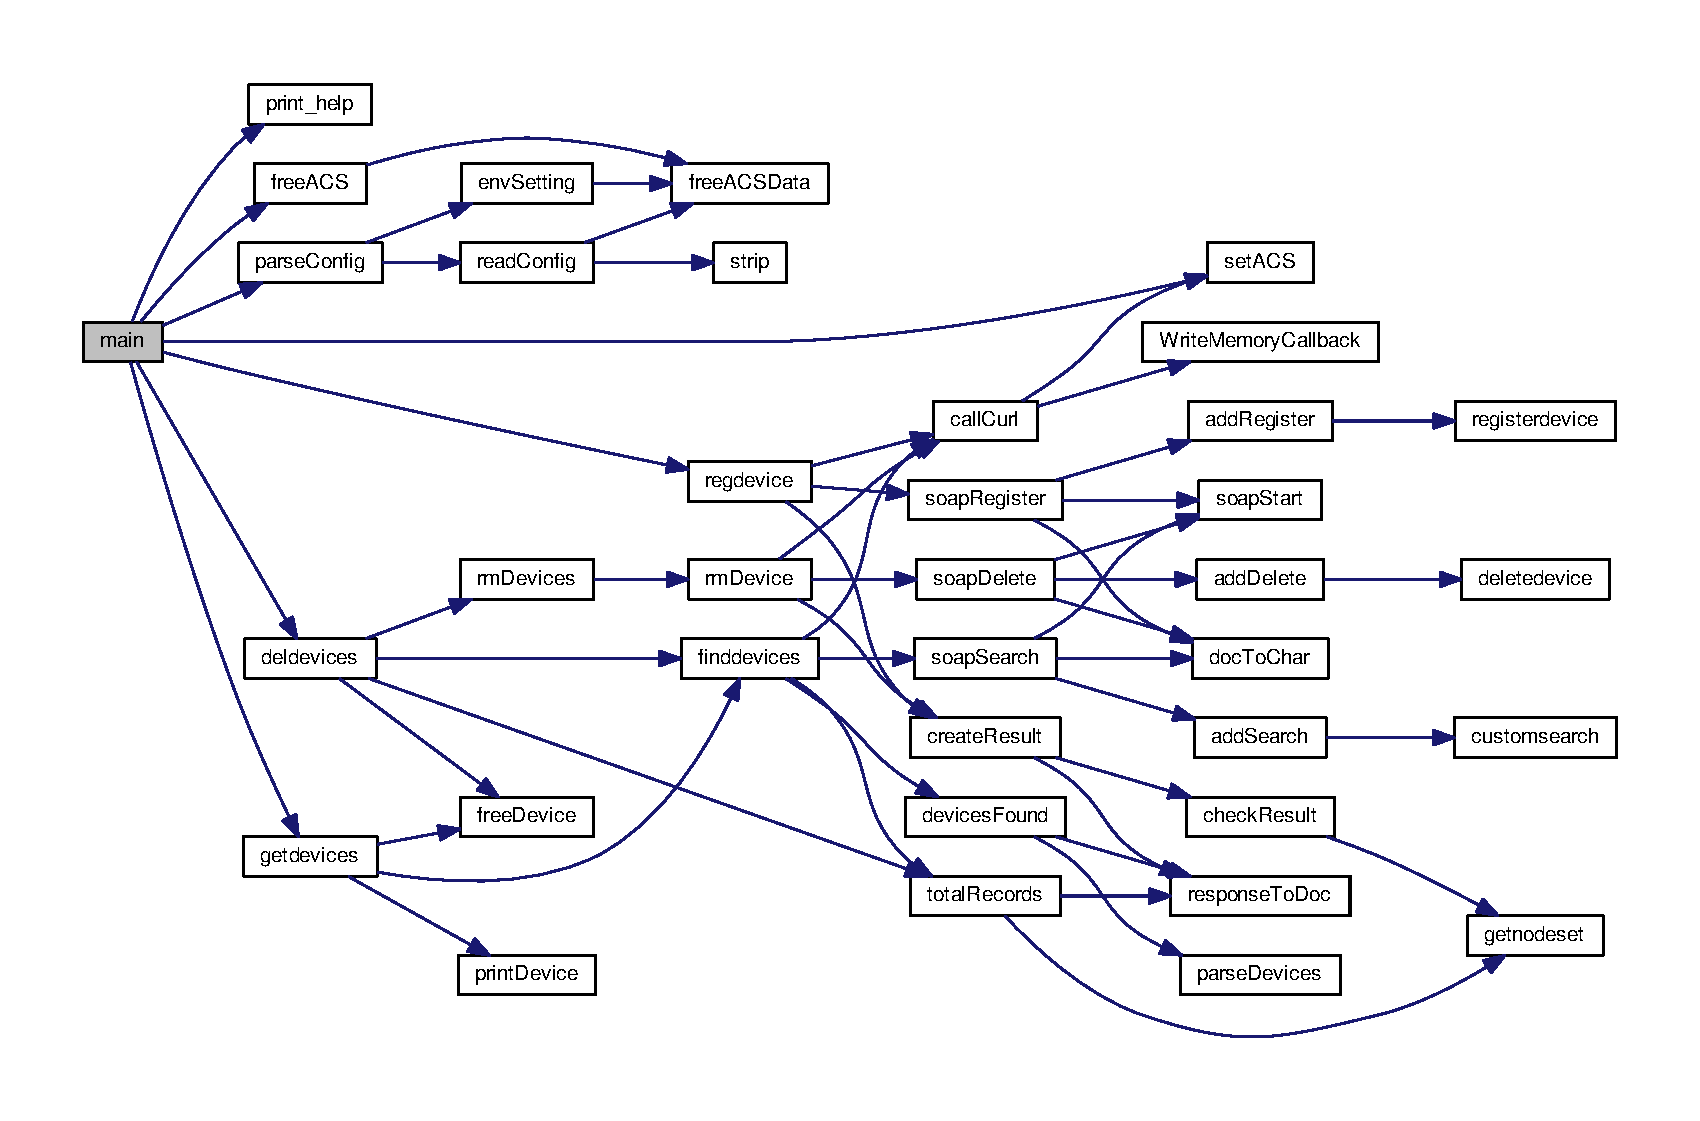
\includegraphics[width=350pt]{ancle_8c_a3c04138a5bfe5d72780bb7e82a18e627_cgraph}
\end{center}
\end{figure}


\hypertarget{ancle_8c_a853216ac51aa181669ff4d3de74058a7}{\index{ancle.\-c@{ancle.\-c}!print\-\_\-help@{print\-\_\-help}}
\index{print\-\_\-help@{print\-\_\-help}!ancle.c@{ancle.\-c}}
\subsubsection[{print\-\_\-help}]{\setlength{\rightskip}{0pt plus 5cm}void print\-\_\-help (
\begin{DoxyParamCaption}
{}
\end{DoxyParamCaption}
)}}\label{ancle_8c_a853216ac51aa181669ff4d3de74058a7}
Print help message to the console 

Definition at line 55 of file ancle.\-c.



\subsection{Variable Documentation}
\hypertarget{ancle_8c_a0b2caeb4b6f130be43e5a2f0267dd453}{\index{ancle.\-c@{ancle.\-c}!verbose@{verbose}}
\index{verbose@{verbose}!ancle.c@{ancle.\-c}}
\subsubsection[{verbose}]{\setlength{\rightskip}{0pt plus 5cm}int verbose = 0}}\label{ancle_8c_a0b2caeb4b6f130be43e5a2f0267dd453}
Verbose switch. If set to 1, program will output debug informations to the standard output 

Definition at line 42 of file ancle.\-c.

\hypertarget{ancle_8c_a7716c14cb5f92e9c141cdec3b980fa70}{\index{ancle.\-c@{ancle.\-c}!yes@{yes}}
\index{yes@{yes}!ancle.c@{ancle.\-c}}
\subsubsection[{yes}]{\setlength{\rightskip}{0pt plus 5cm}int yes = 0}}\label{ancle_8c_a7716c14cb5f92e9c141cdec3b980fa70}
Assume yes switch. If set to 1, program will assume yes on all promits and skip them. 

Definition at line 48 of file ancle.\-c.


\hypertarget{ancle_8h}{\section{src/ancle.h File Reference}
\label{ancle_8h}\index{src/ancle.\-h@{src/ancle.\-h}}
}


main header file for A\-N\-C\-L\-E  


{\ttfamily \#include $<$libxml/parser.\-h$>$}\\*
Include dependency graph for ancle.\-h\-:\nopagebreak
\begin{figure}[H]
\begin{center}
\leavevmode
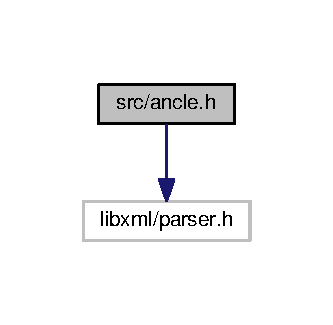
\includegraphics[width=160pt]{ancle_8h__incl}
\end{center}
\end{figure}
This graph shows which files directly or indirectly include this file\-:\nopagebreak
\begin{figure}[H]
\begin{center}
\leavevmode
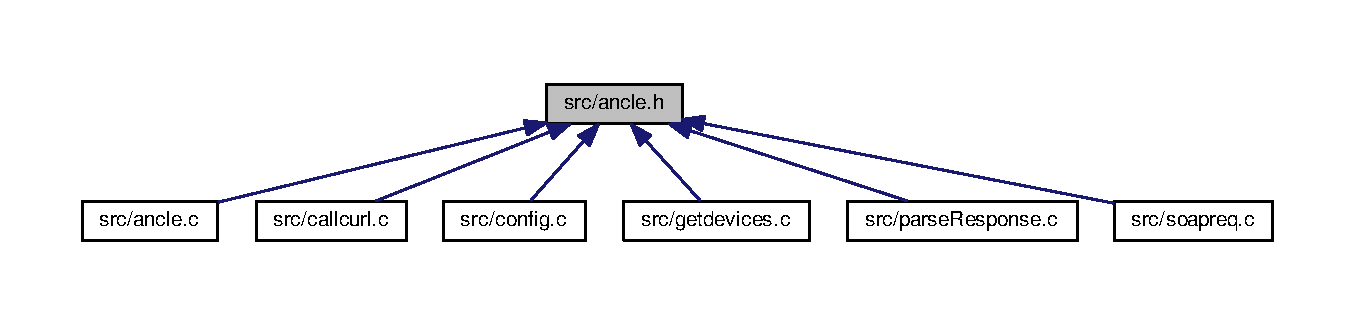
\includegraphics[width=350pt]{ancle_8h__dep__incl}
\end{center}
\end{figure}
\subsection*{Data Structures}
\begin{DoxyCompactItemize}
\item 
struct \hyperlink{structMemoryStruct}{Memory\-Struct}
\item 
struct \hyperlink{structDeviceStruct}{Device\-Struct}
\item 
struct \hyperlink{structacsdata}{acsdata}
\end{DoxyCompactItemize}
\subsection*{Macros}
\begin{DoxyCompactItemize}
\item 
\#define \hyperlink{ancle_8h_a2dfb0858fba4e613654334d012a26483}{A\-C\-S\-\_\-\-N\-B\-I\-\_\-\-U\-R\-L}~\char`\"{}http\-://l01acslab.\-ot.\-hr/nbi.\-php\char`\"{}
\item 
\#define \hyperlink{ancle_8h_ae75670fe5876d9a07090c093f223a2af}{A\-C\-S\-\_\-\-N\-B\-I\-\_\-\-U\-S\-E\-R\-P\-W\-D}~\char`\"{}nbiuser\-:nbipass\char`\"{}
\item 
\#define \hyperlink{ancle_8h_a1a3381cd0df02f019e9ff312091a388e}{L\-O\-C\-A\-L\-\_\-\-C\-O\-N\-F\-I\-G}~\char`\"{}/.anclerc\char`\"{}
\item 
\#define \hyperlink{ancle_8h_a851f17c8aac628fa4054b923a3f9218a}{G\-L\-O\-B\-A\-L\-\_\-\-C\-O\-N\-F\-I\-G}~\char`\"{}/etc/anclerc\char`\"{}
\end{DoxyCompactItemize}
\subsection*{Typedefs}
\begin{DoxyCompactItemize}
\item 
typedef struct \hyperlink{structDeviceStruct}{Device\-Struct} \hyperlink{ancle_8h_a6a13e1aa33261886e04371dfaa52d523}{Device}
\item 
typedef \hyperlink{ancle_8h_a6a13e1aa33261886e04371dfaa52d523}{Device} $\ast$ \hyperlink{ancle_8h_aead9b1579971376ebe2b29db3aacec7a}{Device\-Ptr}
\item 
typedef struct \hyperlink{structacsdata}{acsdata} \hyperlink{ancle_8h_a5ed88d98ea3988cba314b8b251c219ad}{acs}
\end{DoxyCompactItemize}
\subsection*{Functions}
\begin{DoxyCompactItemize}
\item 
int \hyperlink{ancle_8h_a0ea5ed437e02e57952c2302ba96adce0}{getdevices} (\hyperlink{ancle_8h_a6a13e1aa33261886e04371dfaa52d523}{Device} $\ast$device)
\begin{DoxyCompactList}\small\item\em Find devices based on parameter and display it. \end{DoxyCompactList}\item 
int \hyperlink{ancle_8h_afd2f9995728ed462a9e6c694a724eea8}{deldevices} (\hyperlink{ancle_8h_a6a13e1aa33261886e04371dfaa52d523}{Device} $\ast$device)
\item 
int \hyperlink{ancle_8h_aae5f3a031a7b5db1dc464bfbeb8a4f14}{regdevice} (\hyperlink{ancle_8h_a6a13e1aa33261886e04371dfaa52d523}{Device} $\ast$device)
\item 
int \hyperlink{ancle_8h_ad8651923e11cb43708fd39c49eebdf0a}{call\-Curl} (char $\ast$request, struct \hyperlink{structMemoryStruct}{Memory\-Struct} $\ast$response)
\item 
char $\ast$ \hyperlink{ancle_8h_aa41a6f9e907badaf2f5e79a4873b100d}{soap\-Search} (\hyperlink{ancle_8h_aead9b1579971376ebe2b29db3aacec7a}{Device\-Ptr} dev)
\item 
char $\ast$ \hyperlink{ancle_8h_ab45638d882a6836701b6afc3afa64c83}{soap\-Register} (\hyperlink{ancle_8h_aead9b1579971376ebe2b29db3aacec7a}{Device\-Ptr} dev)
\item 
char $\ast$ \hyperlink{ancle_8h_ae4dfd1828415dc5cd6480501dc30cebb}{soap\-Delete} (\hyperlink{ancle_8h_aead9b1579971376ebe2b29db3aacec7a}{Device\-Ptr} dev)
\item 
int \hyperlink{ancle_8h_a3b80bdc3ecd85632e86c4b286a9ae0cb}{total\-Records} (char $\ast$response)
\item 
\hyperlink{ancle_8h_a6a13e1aa33261886e04371dfaa52d523}{Device} $\ast$ \hyperlink{ancle_8h_a2ff61ace0f1a1cc1f7264758b5628152}{devices\-Found} (char $\ast$response, int total)
\item 
void \hyperlink{ancle_8h_a394816653aa6d95dc72852c256d6ba5d}{free\-Device} (\hyperlink{ancle_8h_a6a13e1aa33261886e04371dfaa52d523}{Device} $\ast$device\-List)
\item 
void \hyperlink{ancle_8h_a7934291746b2e8dfed15ffb92af49abd}{print\-Device} (\hyperlink{ancle_8h_a6a13e1aa33261886e04371dfaa52d523}{Device} $\ast$device\-List)
\item 
xml\-Char $\ast$ \hyperlink{ancle_8h_a1c9c9a63964a0d0f06e35ce4cba3006d}{create\-Result} (char $\ast$response)
\item 
void \hyperlink{ancle_8h_a14b70343e2bb126c728f3ad5e93cdd4d}{free\-A\-C\-S} (\hyperlink{ancle_8h_a5ed88d98ea3988cba314b8b251c219ad}{acs} $\ast$\hyperlink{config_8c_ad5fc7e01a4bb3aede66e4f99d8095724}{serverdata})
\item 
int \hyperlink{ancle_8h_a6f119b6d25f7c3bf2c8aa4770f580a95}{parse\-Config} (char $\ast$user\-Config\-File)
\item 
\hyperlink{ancle_8h_a5ed88d98ea3988cba314b8b251c219ad}{acs} $\ast$ \hyperlink{ancle_8h_ad9a110009547c176b81af6d519486337}{set\-A\-C\-S} ()
\end{DoxyCompactItemize}
\subsection*{Variables}
\begin{DoxyCompactItemize}
\item 
int \hyperlink{ancle_8h_a0b2caeb4b6f130be43e5a2f0267dd453}{verbose}
\item 
int \hyperlink{ancle_8h_a7716c14cb5f92e9c141cdec3b980fa70}{yes}
\end{DoxyCompactItemize}


\subsection{Detailed Description}
main header file for A\-N\-C\-L\-E File contains funcion, globals, definitions and macros for Ancle program 

Definition in file \hyperlink{ancle_8h_source}{ancle.\-h}.



\subsection{Macro Definition Documentation}
\hypertarget{ancle_8h_a2dfb0858fba4e613654334d012a26483}{\index{ancle.\-h@{ancle.\-h}!A\-C\-S\-\_\-\-N\-B\-I\-\_\-\-U\-R\-L@{A\-C\-S\-\_\-\-N\-B\-I\-\_\-\-U\-R\-L}}
\index{A\-C\-S\-\_\-\-N\-B\-I\-\_\-\-U\-R\-L@{A\-C\-S\-\_\-\-N\-B\-I\-\_\-\-U\-R\-L}!ancle.h@{ancle.\-h}}
\subsubsection[{A\-C\-S\-\_\-\-N\-B\-I\-\_\-\-U\-R\-L}]{\setlength{\rightskip}{0pt plus 5cm}\#define A\-C\-S\-\_\-\-N\-B\-I\-\_\-\-U\-R\-L~\char`\"{}http\-://l01acslab.\-ot.\-hr/nbi.\-php\char`\"{}}}\label{ancle_8h_a2dfb0858fba4e613654334d012a26483}


Definition at line 32 of file ancle.\-h.

\hypertarget{ancle_8h_ae75670fe5876d9a07090c093f223a2af}{\index{ancle.\-h@{ancle.\-h}!A\-C\-S\-\_\-\-N\-B\-I\-\_\-\-U\-S\-E\-R\-P\-W\-D@{A\-C\-S\-\_\-\-N\-B\-I\-\_\-\-U\-S\-E\-R\-P\-W\-D}}
\index{A\-C\-S\-\_\-\-N\-B\-I\-\_\-\-U\-S\-E\-R\-P\-W\-D@{A\-C\-S\-\_\-\-N\-B\-I\-\_\-\-U\-S\-E\-R\-P\-W\-D}!ancle.h@{ancle.\-h}}
\subsubsection[{A\-C\-S\-\_\-\-N\-B\-I\-\_\-\-U\-S\-E\-R\-P\-W\-D}]{\setlength{\rightskip}{0pt plus 5cm}\#define A\-C\-S\-\_\-\-N\-B\-I\-\_\-\-U\-S\-E\-R\-P\-W\-D~\char`\"{}nbiuser\-:nbipass\char`\"{}}}\label{ancle_8h_ae75670fe5876d9a07090c093f223a2af}


Definition at line 33 of file ancle.\-h.

\hypertarget{ancle_8h_a851f17c8aac628fa4054b923a3f9218a}{\index{ancle.\-h@{ancle.\-h}!G\-L\-O\-B\-A\-L\-\_\-\-C\-O\-N\-F\-I\-G@{G\-L\-O\-B\-A\-L\-\_\-\-C\-O\-N\-F\-I\-G}}
\index{G\-L\-O\-B\-A\-L\-\_\-\-C\-O\-N\-F\-I\-G@{G\-L\-O\-B\-A\-L\-\_\-\-C\-O\-N\-F\-I\-G}!ancle.h@{ancle.\-h}}
\subsubsection[{G\-L\-O\-B\-A\-L\-\_\-\-C\-O\-N\-F\-I\-G}]{\setlength{\rightskip}{0pt plus 5cm}\#define G\-L\-O\-B\-A\-L\-\_\-\-C\-O\-N\-F\-I\-G~\char`\"{}/etc/anclerc\char`\"{}}}\label{ancle_8h_a851f17c8aac628fa4054b923a3f9218a}
define global configuration file 

Definition at line 42 of file ancle.\-h.

\hypertarget{ancle_8h_a1a3381cd0df02f019e9ff312091a388e}{\index{ancle.\-h@{ancle.\-h}!L\-O\-C\-A\-L\-\_\-\-C\-O\-N\-F\-I\-G@{L\-O\-C\-A\-L\-\_\-\-C\-O\-N\-F\-I\-G}}
\index{L\-O\-C\-A\-L\-\_\-\-C\-O\-N\-F\-I\-G@{L\-O\-C\-A\-L\-\_\-\-C\-O\-N\-F\-I\-G}!ancle.h@{ancle.\-h}}
\subsubsection[{L\-O\-C\-A\-L\-\_\-\-C\-O\-N\-F\-I\-G}]{\setlength{\rightskip}{0pt plus 5cm}\#define L\-O\-C\-A\-L\-\_\-\-C\-O\-N\-F\-I\-G~\char`\"{}/.anclerc\char`\"{}}}\label{ancle_8h_a1a3381cd0df02f019e9ff312091a388e}
define user's configuration file 

Definition at line 38 of file ancle.\-h.



\subsection{Typedef Documentation}
\hypertarget{ancle_8h_a5ed88d98ea3988cba314b8b251c219ad}{\index{ancle.\-h@{ancle.\-h}!acs@{acs}}
\index{acs@{acs}!ancle.h@{ancle.\-h}}
\subsubsection[{acs}]{\setlength{\rightskip}{0pt plus 5cm}typedef struct {\bf acsdata}  {\bf acs}}}\label{ancle_8h_a5ed88d98ea3988cba314b8b251c219ad}
A\-C\-S server data \hypertarget{ancle_8h_a6a13e1aa33261886e04371dfaa52d523}{\index{ancle.\-h@{ancle.\-h}!Device@{Device}}
\index{Device@{Device}!ancle.h@{ancle.\-h}}
\subsubsection[{Device}]{\setlength{\rightskip}{0pt plus 5cm}typedef struct {\bf Device\-Struct}  {\bf Device}}}\label{ancle_8h_a6a13e1aa33261886e04371dfaa52d523}
Basic device structure

Maximum string size (without null) is 64 bytes for every member of the structure exept oui which is 6 \hypertarget{ancle_8h_aead9b1579971376ebe2b29db3aacec7a}{\index{ancle.\-h@{ancle.\-h}!Device\-Ptr@{Device\-Ptr}}
\index{Device\-Ptr@{Device\-Ptr}!ancle.h@{ancle.\-h}}
\subsubsection[{Device\-Ptr}]{\setlength{\rightskip}{0pt plus 5cm}typedef {\bf Device}$\ast$ {\bf Device\-Ptr}}}\label{ancle_8h_aead9b1579971376ebe2b29db3aacec7a}
Define Pointer for Device structure 

Definition at line 71 of file ancle.\-h.



\subsection{Function Documentation}
\hypertarget{ancle_8h_ad8651923e11cb43708fd39c49eebdf0a}{\index{ancle.\-h@{ancle.\-h}!call\-Curl@{call\-Curl}}
\index{call\-Curl@{call\-Curl}!ancle.h@{ancle.\-h}}
\subsubsection[{call\-Curl}]{\setlength{\rightskip}{0pt plus 5cm}int call\-Curl (
\begin{DoxyParamCaption}
\item[{char $\ast$}]{request, }
\item[{struct {\bf Memory\-Struct} $\ast$}]{response}
\end{DoxyParamCaption}
)}}\label{ancle_8h_ad8651923e11cb43708fd39c49eebdf0a}


Definition at line 47 of file callcurl.\-c.



Here is the call graph for this function\-:\nopagebreak
\begin{figure}[H]
\begin{center}
\leavevmode
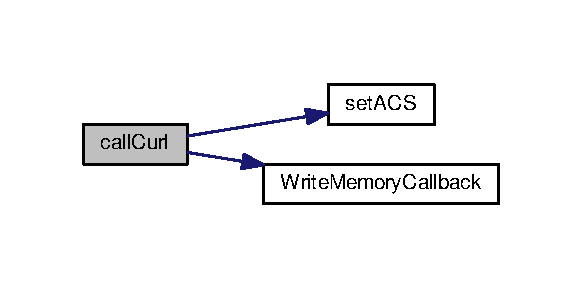
\includegraphics[width=280pt]{ancle_8h_ad8651923e11cb43708fd39c49eebdf0a_cgraph}
\end{center}
\end{figure}


\hypertarget{ancle_8h_a1c9c9a63964a0d0f06e35ce4cba3006d}{\index{ancle.\-h@{ancle.\-h}!create\-Result@{create\-Result}}
\index{create\-Result@{create\-Result}!ancle.h@{ancle.\-h}}
\subsubsection[{create\-Result}]{\setlength{\rightskip}{0pt plus 5cm}xml\-Char$\ast$ create\-Result (
\begin{DoxyParamCaption}
\item[{char $\ast$}]{response}
\end{DoxyParamCaption}
)}}\label{ancle_8h_a1c9c9a63964a0d0f06e35ce4cba3006d}


Definition at line 150 of file parse\-Response.\-c.



Here is the call graph for this function\-:\nopagebreak
\begin{figure}[H]
\begin{center}
\leavevmode
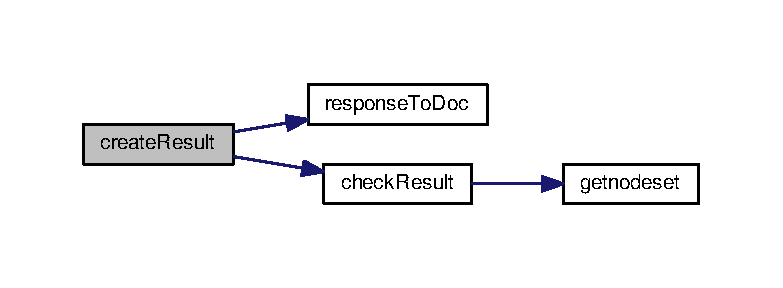
\includegraphics[width=350pt]{ancle_8h_a1c9c9a63964a0d0f06e35ce4cba3006d_cgraph}
\end{center}
\end{figure}


\hypertarget{ancle_8h_afd2f9995728ed462a9e6c694a724eea8}{\index{ancle.\-h@{ancle.\-h}!deldevices@{deldevices}}
\index{deldevices@{deldevices}!ancle.h@{ancle.\-h}}
\subsubsection[{deldevices}]{\setlength{\rightskip}{0pt plus 5cm}int deldevices (
\begin{DoxyParamCaption}
\item[{{\bf Device} $\ast$}]{device}
\end{DoxyParamCaption}
)}}\label{ancle_8h_afd2f9995728ed462a9e6c694a724eea8}
Delete devices based on search paramter delete is yet not completed and will act as getdevices function 
\begin{DoxyParams}{Parameters}
{\em device} & reference device that will used as search pattern \\
\hline
\end{DoxyParams}


Definition at line 178 of file getdevices.\-c.



Here is the call graph for this function\-:\nopagebreak
\begin{figure}[H]
\begin{center}
\leavevmode
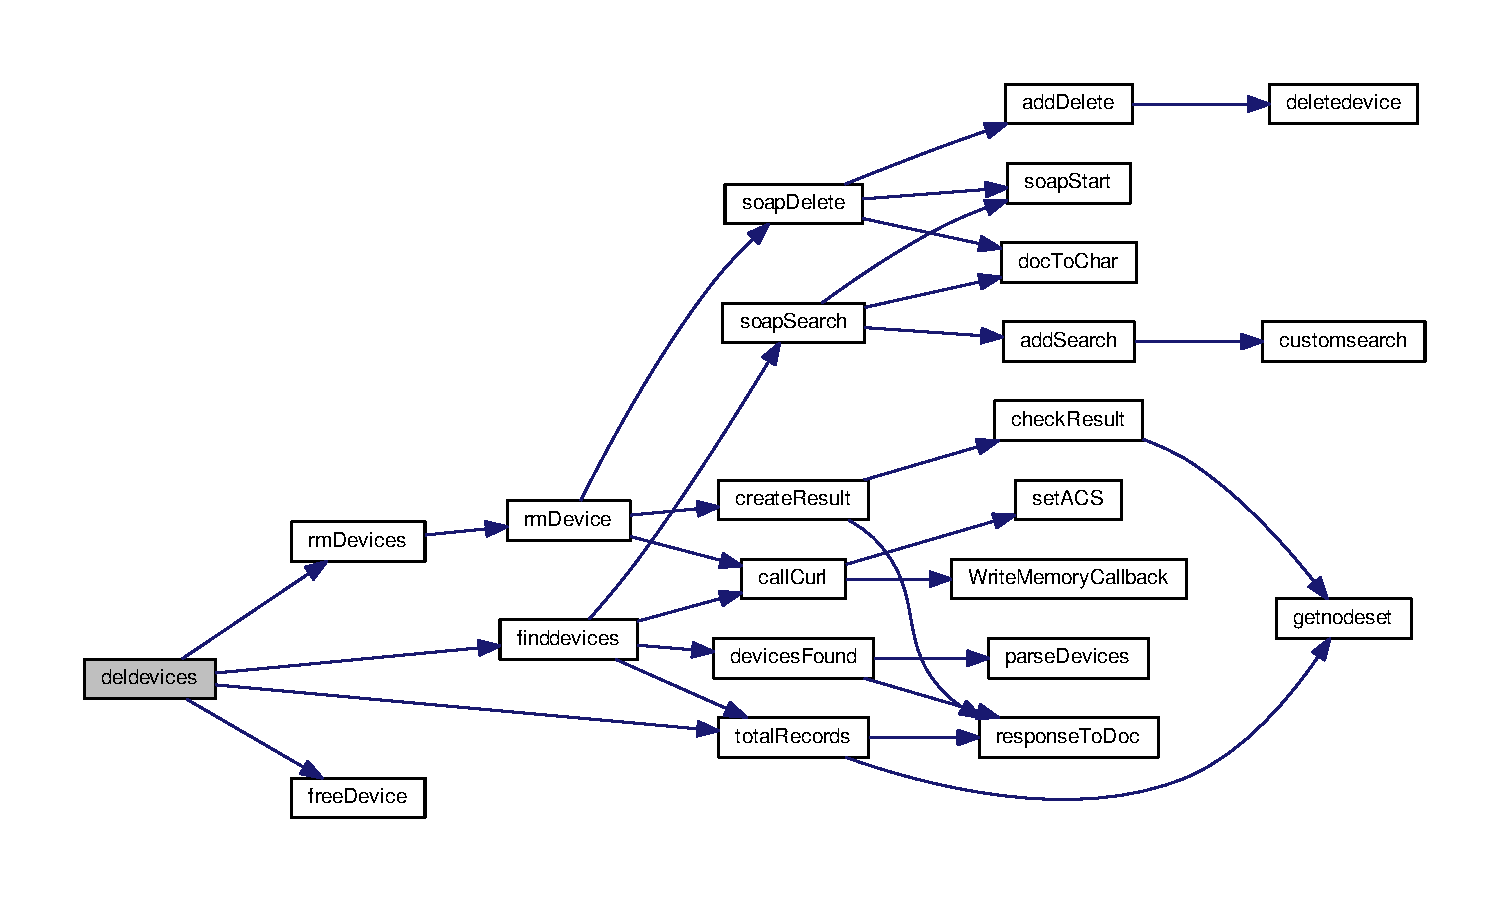
\includegraphics[width=350pt]{ancle_8h_afd2f9995728ed462a9e6c694a724eea8_cgraph}
\end{center}
\end{figure}


\hypertarget{ancle_8h_a2ff61ace0f1a1cc1f7264758b5628152}{\index{ancle.\-h@{ancle.\-h}!devices\-Found@{devices\-Found}}
\index{devices\-Found@{devices\-Found}!ancle.h@{ancle.\-h}}
\subsubsection[{devices\-Found}]{\setlength{\rightskip}{0pt plus 5cm}{\bf Device}$\ast$ devices\-Found (
\begin{DoxyParamCaption}
\item[{char $\ast$}]{response, }
\item[{int}]{total}
\end{DoxyParamCaption}
)}}\label{ancle_8h_a2ff61ace0f1a1cc1f7264758b5628152}


Definition at line 272 of file parse\-Response.\-c.



Here is the call graph for this function\-:\nopagebreak
\begin{figure}[H]
\begin{center}
\leavevmode
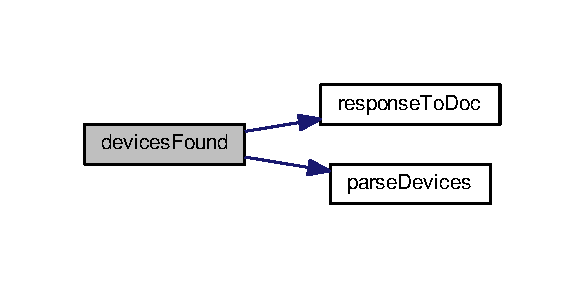
\includegraphics[width=280pt]{ancle_8h_a2ff61ace0f1a1cc1f7264758b5628152_cgraph}
\end{center}
\end{figure}


\hypertarget{ancle_8h_a14b70343e2bb126c728f3ad5e93cdd4d}{\index{ancle.\-h@{ancle.\-h}!free\-A\-C\-S@{free\-A\-C\-S}}
\index{free\-A\-C\-S@{free\-A\-C\-S}!ancle.h@{ancle.\-h}}
\subsubsection[{free\-A\-C\-S}]{\setlength{\rightskip}{0pt plus 5cm}void free\-A\-C\-S (
\begin{DoxyParamCaption}
\item[{{\bf acs} $\ast$}]{serverdata}
\end{DoxyParamCaption}
)}}\label{ancle_8h_a14b70343e2bb126c728f3ad5e93cdd4d}


Definition at line 104 of file config.\-c.



Here is the call graph for this function\-:\nopagebreak
\begin{figure}[H]
\begin{center}
\leavevmode
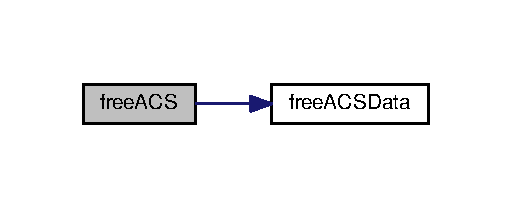
\includegraphics[width=246pt]{ancle_8h_a14b70343e2bb126c728f3ad5e93cdd4d_cgraph}
\end{center}
\end{figure}


\hypertarget{ancle_8h_a394816653aa6d95dc72852c256d6ba5d}{\index{ancle.\-h@{ancle.\-h}!free\-Device@{free\-Device}}
\index{free\-Device@{free\-Device}!ancle.h@{ancle.\-h}}
\subsubsection[{free\-Device}]{\setlength{\rightskip}{0pt plus 5cm}void free\-Device (
\begin{DoxyParamCaption}
\item[{{\bf Device} $\ast$}]{device\-List}
\end{DoxyParamCaption}
)}}\label{ancle_8h_a394816653aa6d95dc72852c256d6ba5d}


Definition at line 41 of file parse\-Response.\-c.

\hypertarget{ancle_8h_a0ea5ed437e02e57952c2302ba96adce0}{\index{ancle.\-h@{ancle.\-h}!getdevices@{getdevices}}
\index{getdevices@{getdevices}!ancle.h@{ancle.\-h}}
\subsubsection[{getdevices}]{\setlength{\rightskip}{0pt plus 5cm}int getdevices (
\begin{DoxyParamCaption}
\item[{{\bf Device} $\ast$}]{device}
\end{DoxyParamCaption}
)}}\label{ancle_8h_a0ea5ed437e02e57952c2302ba96adce0}


Find devices based on parameter and display it. 

Global functions


\begin{DoxyParams}{Parameters}
{\em device} & reference device that will used as search pattern \\
\hline
\end{DoxyParams}


Definition at line 92 of file getdevices.\-c.



Here is the call graph for this function\-:\nopagebreak
\begin{figure}[H]
\begin{center}
\leavevmode
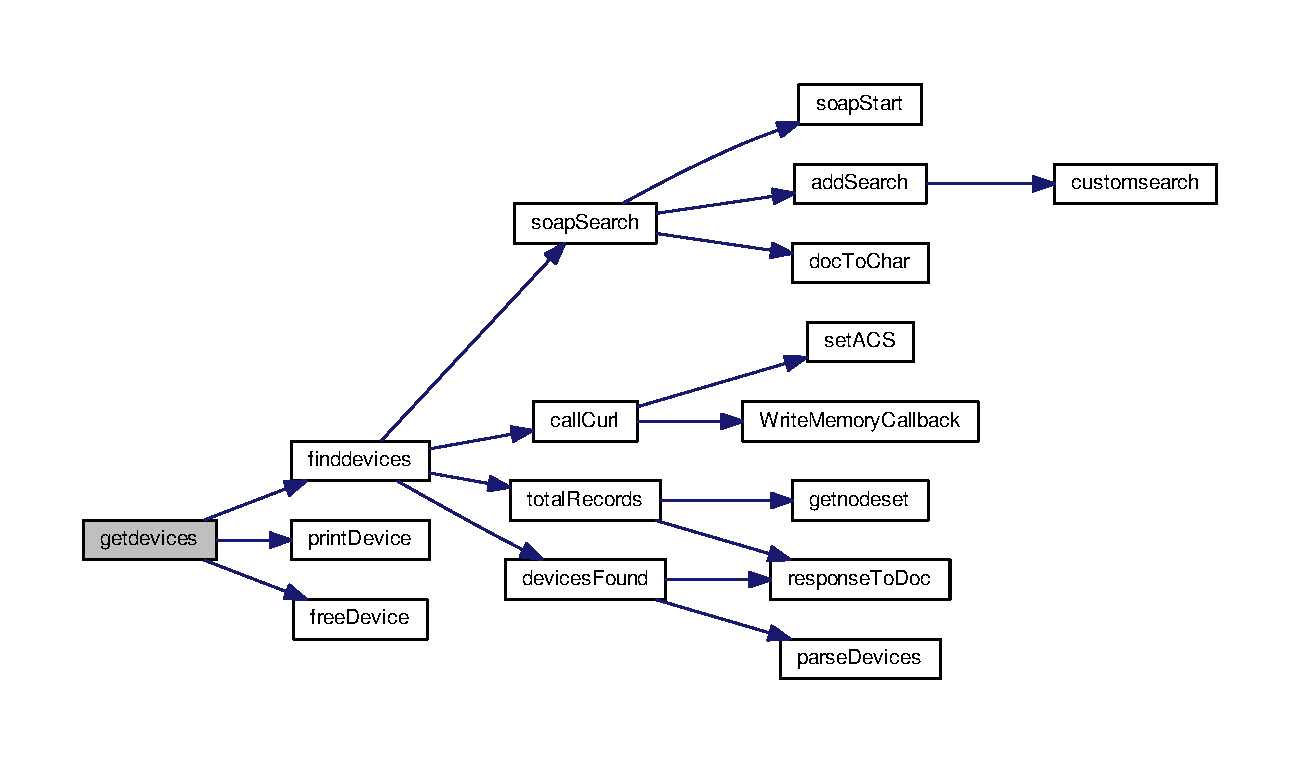
\includegraphics[width=350pt]{ancle_8h_a0ea5ed437e02e57952c2302ba96adce0_cgraph}
\end{center}
\end{figure}


\hypertarget{ancle_8h_a6f119b6d25f7c3bf2c8aa4770f580a95}{\index{ancle.\-h@{ancle.\-h}!parse\-Config@{parse\-Config}}
\index{parse\-Config@{parse\-Config}!ancle.h@{ancle.\-h}}
\subsubsection[{parse\-Config}]{\setlength{\rightskip}{0pt plus 5cm}int parse\-Config (
\begin{DoxyParamCaption}
\item[{char $\ast$}]{user\-Config\-File}
\end{DoxyParamCaption}
)}}\label{ancle_8h_a6f119b6d25f7c3bf2c8aa4770f580a95}


Definition at line 53 of file config.\-c.



Here is the call graph for this function\-:\nopagebreak
\begin{figure}[H]
\begin{center}
\leavevmode
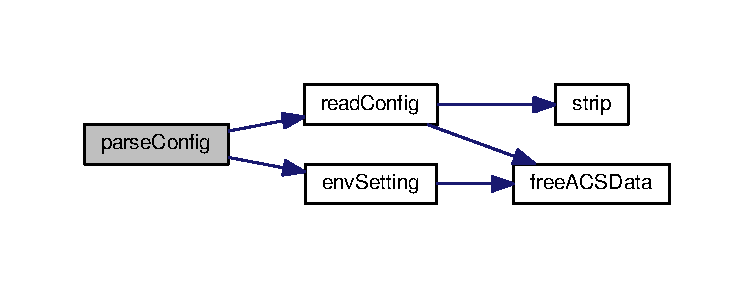
\includegraphics[width=350pt]{ancle_8h_a6f119b6d25f7c3bf2c8aa4770f580a95_cgraph}
\end{center}
\end{figure}


\hypertarget{ancle_8h_a7934291746b2e8dfed15ffb92af49abd}{\index{ancle.\-h@{ancle.\-h}!print\-Device@{print\-Device}}
\index{print\-Device@{print\-Device}!ancle.h@{ancle.\-h}}
\subsubsection[{print\-Device}]{\setlength{\rightskip}{0pt plus 5cm}void print\-Device (
\begin{DoxyParamCaption}
\item[{{\bf Device} $\ast$}]{device\-List}
\end{DoxyParamCaption}
)}}\label{ancle_8h_a7934291746b2e8dfed15ffb92af49abd}


Definition at line 56 of file parse\-Response.\-c.

\hypertarget{ancle_8h_aae5f3a031a7b5db1dc464bfbeb8a4f14}{\index{ancle.\-h@{ancle.\-h}!regdevice@{regdevice}}
\index{regdevice@{regdevice}!ancle.h@{ancle.\-h}}
\subsubsection[{regdevice}]{\setlength{\rightskip}{0pt plus 5cm}int regdevice (
\begin{DoxyParamCaption}
\item[{{\bf Device} $\ast$}]{device}
\end{DoxyParamCaption}
)}}\label{ancle_8h_aae5f3a031a7b5db1dc464bfbeb8a4f14}
Used to register new device into A\-C\-S server 
\begin{DoxyParams}{Parameters}
{\em device} & must contain fully specified device \\
\hline
\end{DoxyParams}


Definition at line 213 of file getdevices.\-c.



Here is the call graph for this function\-:\nopagebreak
\begin{figure}[H]
\begin{center}
\leavevmode
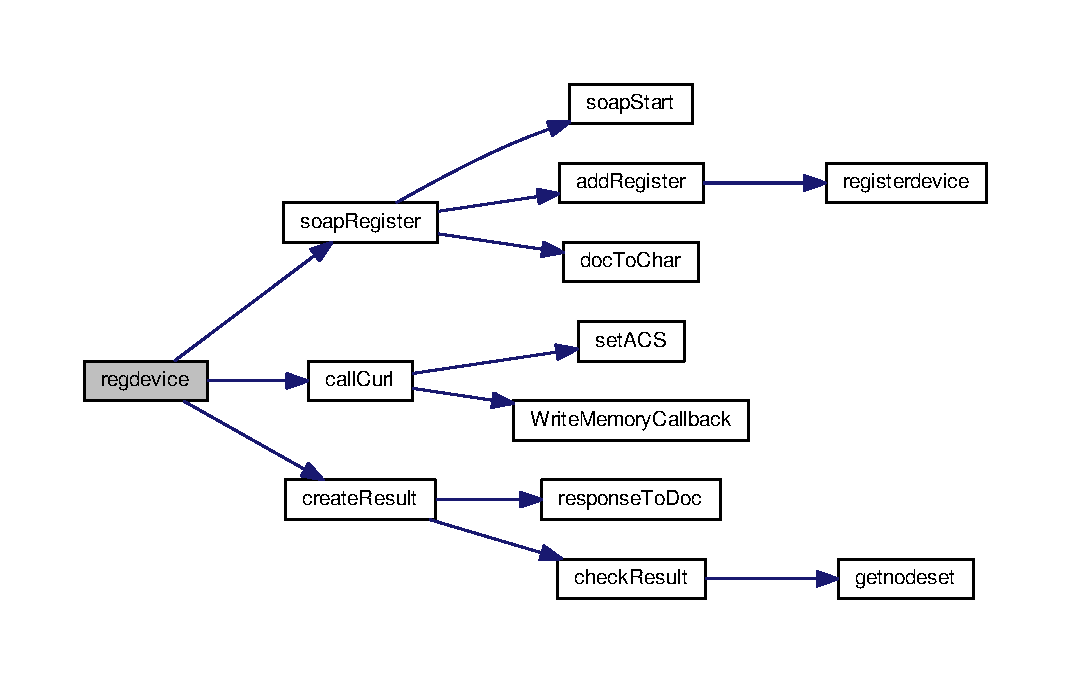
\includegraphics[width=350pt]{ancle_8h_aae5f3a031a7b5db1dc464bfbeb8a4f14_cgraph}
\end{center}
\end{figure}


\hypertarget{ancle_8h_ad9a110009547c176b81af6d519486337}{\index{ancle.\-h@{ancle.\-h}!set\-A\-C\-S@{set\-A\-C\-S}}
\index{set\-A\-C\-S@{set\-A\-C\-S}!ancle.h@{ancle.\-h}}
\subsubsection[{set\-A\-C\-S}]{\setlength{\rightskip}{0pt plus 5cm}{\bf acs}$\ast$ set\-A\-C\-S (
\begin{DoxyParamCaption}
{}
\end{DoxyParamCaption}
)}}\label{ancle_8h_ad9a110009547c176b81af6d519486337}


Definition at line 44 of file config.\-c.

\hypertarget{ancle_8h_ae4dfd1828415dc5cd6480501dc30cebb}{\index{ancle.\-h@{ancle.\-h}!soap\-Delete@{soap\-Delete}}
\index{soap\-Delete@{soap\-Delete}!ancle.h@{ancle.\-h}}
\subsubsection[{soap\-Delete}]{\setlength{\rightskip}{0pt plus 5cm}char$\ast$ soap\-Delete (
\begin{DoxyParamCaption}
\item[{{\bf Device\-Ptr}}]{dev}
\end{DoxyParamCaption}
)}}\label{ancle_8h_ae4dfd1828415dc5cd6480501dc30cebb}


Definition at line 250 of file soapreq.\-c.



Here is the call graph for this function\-:\nopagebreak
\begin{figure}[H]
\begin{center}
\leavevmode
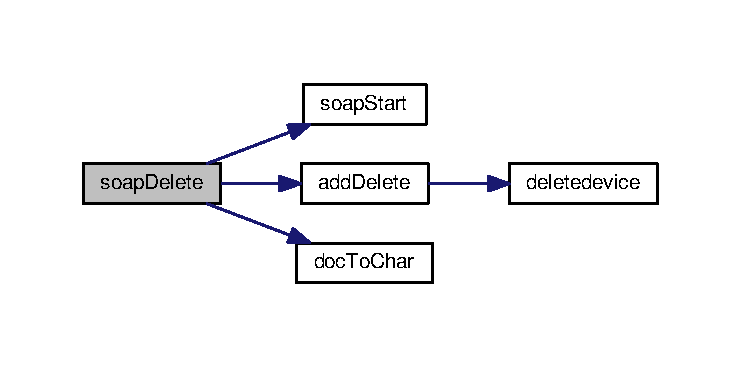
\includegraphics[width=350pt]{ancle_8h_ae4dfd1828415dc5cd6480501dc30cebb_cgraph}
\end{center}
\end{figure}


\hypertarget{ancle_8h_ab45638d882a6836701b6afc3afa64c83}{\index{ancle.\-h@{ancle.\-h}!soap\-Register@{soap\-Register}}
\index{soap\-Register@{soap\-Register}!ancle.h@{ancle.\-h}}
\subsubsection[{soap\-Register}]{\setlength{\rightskip}{0pt plus 5cm}char$\ast$ soap\-Register (
\begin{DoxyParamCaption}
\item[{{\bf Device\-Ptr}}]{dev}
\end{DoxyParamCaption}
)}}\label{ancle_8h_ab45638d882a6836701b6afc3afa64c83}


Definition at line 241 of file soapreq.\-c.



Here is the call graph for this function\-:\nopagebreak
\begin{figure}[H]
\begin{center}
\leavevmode
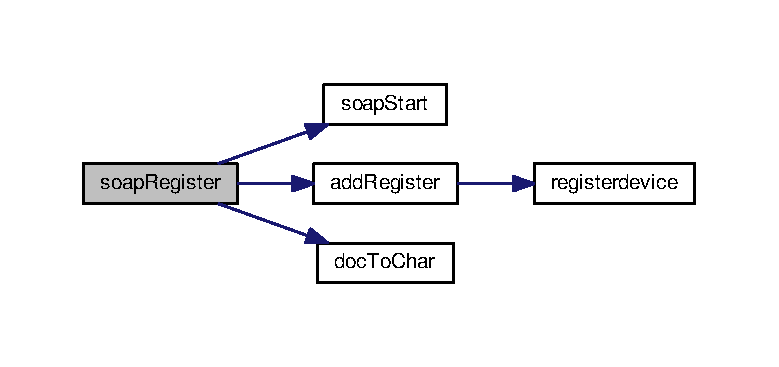
\includegraphics[width=350pt]{ancle_8h_ab45638d882a6836701b6afc3afa64c83_cgraph}
\end{center}
\end{figure}


\hypertarget{ancle_8h_aa41a6f9e907badaf2f5e79a4873b100d}{\index{ancle.\-h@{ancle.\-h}!soap\-Search@{soap\-Search}}
\index{soap\-Search@{soap\-Search}!ancle.h@{ancle.\-h}}
\subsubsection[{soap\-Search}]{\setlength{\rightskip}{0pt plus 5cm}char$\ast$ soap\-Search (
\begin{DoxyParamCaption}
\item[{{\bf Device\-Ptr}}]{dev}
\end{DoxyParamCaption}
)}}\label{ancle_8h_aa41a6f9e907badaf2f5e79a4873b100d}


Definition at line 232 of file soapreq.\-c.



Here is the call graph for this function\-:\nopagebreak
\begin{figure}[H]
\begin{center}
\leavevmode
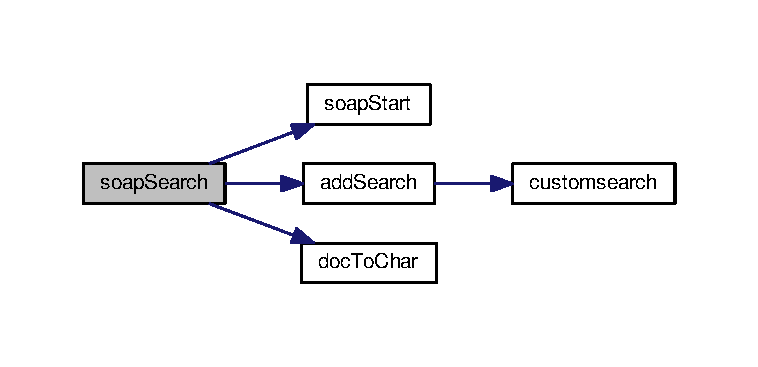
\includegraphics[width=350pt]{ancle_8h_aa41a6f9e907badaf2f5e79a4873b100d_cgraph}
\end{center}
\end{figure}


\hypertarget{ancle_8h_a3b80bdc3ecd85632e86c4b286a9ae0cb}{\index{ancle.\-h@{ancle.\-h}!total\-Records@{total\-Records}}
\index{total\-Records@{total\-Records}!ancle.h@{ancle.\-h}}
\subsubsection[{total\-Records}]{\setlength{\rightskip}{0pt plus 5cm}int total\-Records (
\begin{DoxyParamCaption}
\item[{char $\ast$}]{response}
\end{DoxyParamCaption}
)}}\label{ancle_8h_a3b80bdc3ecd85632e86c4b286a9ae0cb}
Function will parse number of devices from given S\-O\-A\-P response. If response is set to N\-U\-L\-L, then it will return last paresed, nuber of devies 

Definition at line 80 of file parse\-Response.\-c.



Here is the call graph for this function\-:\nopagebreak
\begin{figure}[H]
\begin{center}
\leavevmode
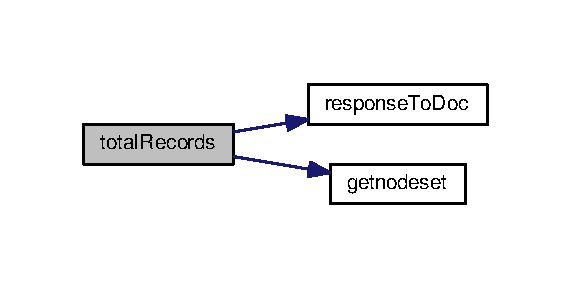
\includegraphics[width=274pt]{ancle_8h_a3b80bdc3ecd85632e86c4b286a9ae0cb_cgraph}
\end{center}
\end{figure}




\subsection{Variable Documentation}
\hypertarget{ancle_8h_a0b2caeb4b6f130be43e5a2f0267dd453}{\index{ancle.\-h@{ancle.\-h}!verbose@{verbose}}
\index{verbose@{verbose}!ancle.h@{ancle.\-h}}
\subsubsection[{verbose}]{\setlength{\rightskip}{0pt plus 5cm}int verbose}}\label{ancle_8h_a0b2caeb4b6f130be43e5a2f0267dd453}
Globals

Verbose switch. If set to 1, program will output debug informations to the standard output 

Definition at line 42 of file ancle.\-c.

\hypertarget{ancle_8h_a7716c14cb5f92e9c141cdec3b980fa70}{\index{ancle.\-h@{ancle.\-h}!yes@{yes}}
\index{yes@{yes}!ancle.h@{ancle.\-h}}
\subsubsection[{yes}]{\setlength{\rightskip}{0pt plus 5cm}int yes}}\label{ancle_8h_a7716c14cb5f92e9c141cdec3b980fa70}
Assume yes switch. If set to 1, program will assume yes on all promits and skip them. 

Definition at line 48 of file ancle.\-c.


\hypertarget{callcurl_8c}{\section{src/callcurl.c File Reference}
\label{callcurl_8c}\index{src/callcurl.\-c@{src/callcurl.\-c}}
}
{\ttfamily \#include $<$stdio.\-h$>$}\\*
{\ttfamily \#include $<$stdlib.\-h$>$}\\*
{\ttfamily \#include $<$string.\-h$>$}\\*
{\ttfamily \#include $<$curl/curl.\-h$>$}\\*
{\ttfamily \#include \char`\"{}ancle.\-h\char`\"{}}\\*
Include dependency graph for callcurl.\-c\-:\nopagebreak
\begin{figure}[H]
\begin{center}
\leavevmode
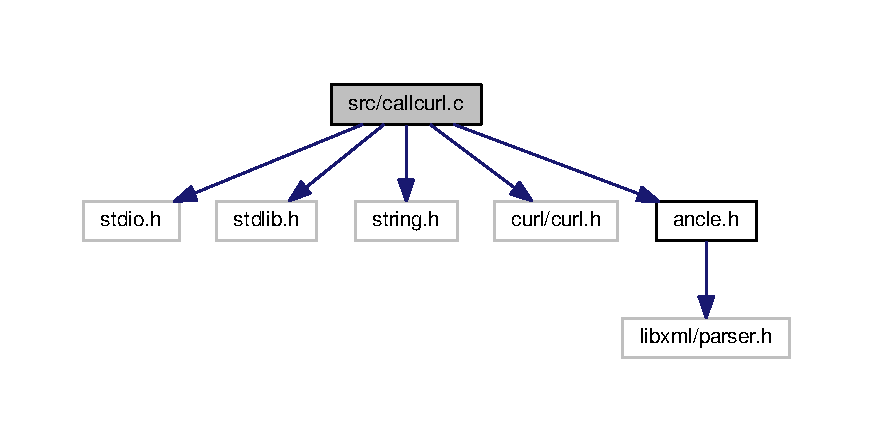
\includegraphics[width=350pt]{callcurl_8c__incl}
\end{center}
\end{figure}
\subsection*{Functions}
\begin{DoxyCompactItemize}
\item 
static size\-\_\-t \hyperlink{callcurl_8c_a4ddd5eda46f8b61317f95145c87e653d}{Write\-Memory\-Callback} (void $\ast$contents, size\-\_\-t size, size\-\_\-t nmemb, void $\ast$userp)
\item 
int \hyperlink{callcurl_8c_ad8651923e11cb43708fd39c49eebdf0a}{call\-Curl} (char $\ast$request, struct \hyperlink{structMemoryStruct}{Memory\-Struct} $\ast$response)
\end{DoxyCompactItemize}


\subsection{Function Documentation}
\hypertarget{callcurl_8c_ad8651923e11cb43708fd39c49eebdf0a}{\index{callcurl.\-c@{callcurl.\-c}!call\-Curl@{call\-Curl}}
\index{call\-Curl@{call\-Curl}!callcurl.c@{callcurl.\-c}}
\subsubsection[{call\-Curl}]{\setlength{\rightskip}{0pt plus 5cm}int call\-Curl (
\begin{DoxyParamCaption}
\item[{char $\ast$}]{request, }
\item[{struct {\bf Memory\-Struct} $\ast$}]{response}
\end{DoxyParamCaption}
)}}\label{callcurl_8c_ad8651923e11cb43708fd39c49eebdf0a}


Definition at line 47 of file callcurl.\-c.



Here is the call graph for this function\-:\nopagebreak
\begin{figure}[H]
\begin{center}
\leavevmode
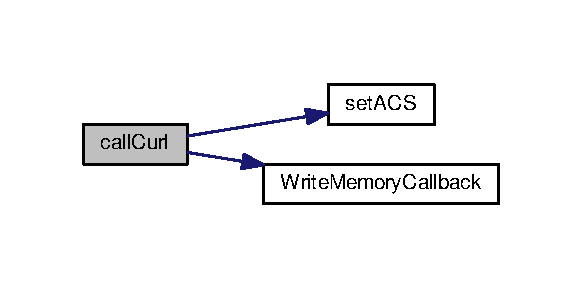
\includegraphics[width=280pt]{callcurl_8c_ad8651923e11cb43708fd39c49eebdf0a_cgraph}
\end{center}
\end{figure}


\hypertarget{callcurl_8c_a4ddd5eda46f8b61317f95145c87e653d}{\index{callcurl.\-c@{callcurl.\-c}!Write\-Memory\-Callback@{Write\-Memory\-Callback}}
\index{Write\-Memory\-Callback@{Write\-Memory\-Callback}!callcurl.c@{callcurl.\-c}}
\subsubsection[{Write\-Memory\-Callback}]{\setlength{\rightskip}{0pt plus 5cm}static size\-\_\-t Write\-Memory\-Callback (
\begin{DoxyParamCaption}
\item[{void $\ast$}]{contents, }
\item[{size\-\_\-t}]{size, }
\item[{size\-\_\-t}]{nmemb, }
\item[{void $\ast$}]{userp}
\end{DoxyParamCaption}
)\hspace{0.3cm}{\ttfamily [static]}}}\label{callcurl_8c_a4ddd5eda46f8b61317f95145c87e653d}


Definition at line 26 of file callcurl.\-c.


\hypertarget{config_8c}{\section{src/config.c File Reference}
\label{config_8c}\index{src/config.\-c@{src/config.\-c}}
}
{\ttfamily \#include $<$stdio.\-h$>$}\\*
{\ttfamily \#include $<$stdlib.\-h$>$}\\*
{\ttfamily \#include $<$string.\-h$>$}\\*
{\ttfamily \#include $<$ctype.\-h$>$}\\*
{\ttfamily \#include $<$errno.\-h$>$}\\*
{\ttfamily \#include \char`\"{}ancle.\-h\char`\"{}}\\*
Include dependency graph for config.\-c\-:\nopagebreak
\begin{figure}[H]
\begin{center}
\leavevmode
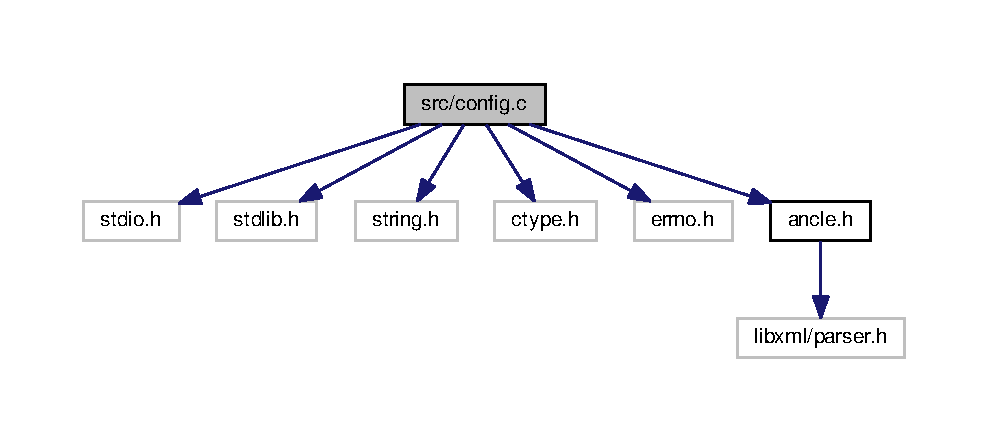
\includegraphics[width=350pt]{config_8c__incl}
\end{center}
\end{figure}
\subsection*{Macros}
\begin{DoxyCompactItemize}
\item 
\#define \hyperlink{config_8c_a3e937c42922f7601edb17b747602c471}{M\-A\-X\-L\-I\-N\-E}~250
\end{DoxyCompactItemize}
\subsection*{Functions}
\begin{DoxyCompactItemize}
\item 
static int \hyperlink{config_8c_a2430ba930020227a368a1aa3bf9ef988}{read\-Config} (char $\ast$filename, \hyperlink{ancle_8h_a5ed88d98ea3988cba314b8b251c219ad}{acs} $\ast$data)
\item 
int \hyperlink{config_8c_aa0a7c2a9082f98e3911b06c6a06fc8bb}{env\-Setting} (\hyperlink{ancle_8h_a5ed88d98ea3988cba314b8b251c219ad}{acs} $\ast$data)
\item 
static void \hyperlink{config_8c_a69763ee67d1bc85f77ea1f7768a137f5}{strip} (char $\ast$string)
\item 
void \hyperlink{config_8c_a6223c55ff47830c4f4cd60e32e4621cc}{free\-A\-C\-S\-Data} (\hyperlink{ancle_8h_a5ed88d98ea3988cba314b8b251c219ad}{acs} $\ast$data)
\item 
\hyperlink{ancle_8h_a5ed88d98ea3988cba314b8b251c219ad}{acs} $\ast$ \hyperlink{config_8c_ad9a110009547c176b81af6d519486337}{set\-A\-C\-S} ()
\item 
int \hyperlink{config_8c_a6f119b6d25f7c3bf2c8aa4770f580a95}{parse\-Config} (char $\ast$user\-Config\-File)
\item 
void \hyperlink{config_8c_a14b70343e2bb126c728f3ad5e93cdd4d}{free\-A\-C\-S} (\hyperlink{ancle_8h_a5ed88d98ea3988cba314b8b251c219ad}{acs} $\ast$\hyperlink{config_8c_ad5fc7e01a4bb3aede66e4f99d8095724}{serverdata})
\end{DoxyCompactItemize}
\subsection*{Variables}
\begin{DoxyCompactItemize}
\item 
static \hyperlink{ancle_8h_a5ed88d98ea3988cba314b8b251c219ad}{acs} $\ast$ \hyperlink{config_8c_ad5fc7e01a4bb3aede66e4f99d8095724}{serverdata}
\end{DoxyCompactItemize}


\subsection{Macro Definition Documentation}
\hypertarget{config_8c_a3e937c42922f7601edb17b747602c471}{\index{config.\-c@{config.\-c}!M\-A\-X\-L\-I\-N\-E@{M\-A\-X\-L\-I\-N\-E}}
\index{M\-A\-X\-L\-I\-N\-E@{M\-A\-X\-L\-I\-N\-E}!config.c@{config.\-c}}
\subsubsection[{M\-A\-X\-L\-I\-N\-E}]{\setlength{\rightskip}{0pt plus 5cm}\#define M\-A\-X\-L\-I\-N\-E~250}}\label{config_8c_a3e937c42922f7601edb17b747602c471}


Definition at line 32 of file config.\-c.



\subsection{Function Documentation}
\hypertarget{config_8c_aa0a7c2a9082f98e3911b06c6a06fc8bb}{\index{config.\-c@{config.\-c}!env\-Setting@{env\-Setting}}
\index{env\-Setting@{env\-Setting}!config.c@{config.\-c}}
\subsubsection[{env\-Setting}]{\setlength{\rightskip}{0pt plus 5cm}int env\-Setting (
\begin{DoxyParamCaption}
\item[{{\bf acs} $\ast$}]{data}
\end{DoxyParamCaption}
)}}\label{config_8c_aa0a7c2a9082f98e3911b06c6a06fc8bb}


Definition at line 112 of file config.\-c.



Here is the call graph for this function\-:\nopagebreak
\begin{figure}[H]
\begin{center}
\leavevmode
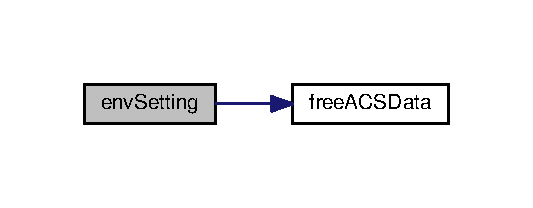
\includegraphics[width=256pt]{config_8c_aa0a7c2a9082f98e3911b06c6a06fc8bb_cgraph}
\end{center}
\end{figure}


\hypertarget{config_8c_a14b70343e2bb126c728f3ad5e93cdd4d}{\index{config.\-c@{config.\-c}!free\-A\-C\-S@{free\-A\-C\-S}}
\index{free\-A\-C\-S@{free\-A\-C\-S}!config.c@{config.\-c}}
\subsubsection[{free\-A\-C\-S}]{\setlength{\rightskip}{0pt plus 5cm}void free\-A\-C\-S (
\begin{DoxyParamCaption}
\item[{{\bf acs} $\ast$}]{serverdata}
\end{DoxyParamCaption}
)}}\label{config_8c_a14b70343e2bb126c728f3ad5e93cdd4d}


Definition at line 104 of file config.\-c.



Here is the call graph for this function\-:\nopagebreak
\begin{figure}[H]
\begin{center}
\leavevmode
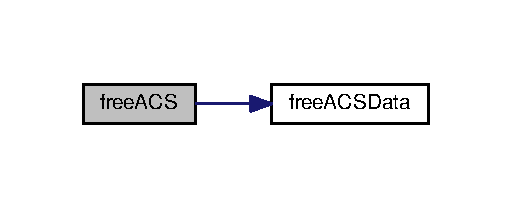
\includegraphics[width=246pt]{config_8c_a14b70343e2bb126c728f3ad5e93cdd4d_cgraph}
\end{center}
\end{figure}


\hypertarget{config_8c_a6223c55ff47830c4f4cd60e32e4621cc}{\index{config.\-c@{config.\-c}!free\-A\-C\-S\-Data@{free\-A\-C\-S\-Data}}
\index{free\-A\-C\-S\-Data@{free\-A\-C\-S\-Data}!config.c@{config.\-c}}
\subsubsection[{free\-A\-C\-S\-Data}]{\setlength{\rightskip}{0pt plus 5cm}void free\-A\-C\-S\-Data (
\begin{DoxyParamCaption}
\item[{{\bf acs} $\ast$}]{data}
\end{DoxyParamCaption}
)}}\label{config_8c_a6223c55ff47830c4f4cd60e32e4621cc}


Definition at line 243 of file config.\-c.

\hypertarget{config_8c_a6f119b6d25f7c3bf2c8aa4770f580a95}{\index{config.\-c@{config.\-c}!parse\-Config@{parse\-Config}}
\index{parse\-Config@{parse\-Config}!config.c@{config.\-c}}
\subsubsection[{parse\-Config}]{\setlength{\rightskip}{0pt plus 5cm}int parse\-Config (
\begin{DoxyParamCaption}
\item[{char $\ast$}]{user\-Config\-File}
\end{DoxyParamCaption}
)}}\label{config_8c_a6f119b6d25f7c3bf2c8aa4770f580a95}


Definition at line 53 of file config.\-c.



Here is the call graph for this function\-:\nopagebreak
\begin{figure}[H]
\begin{center}
\leavevmode
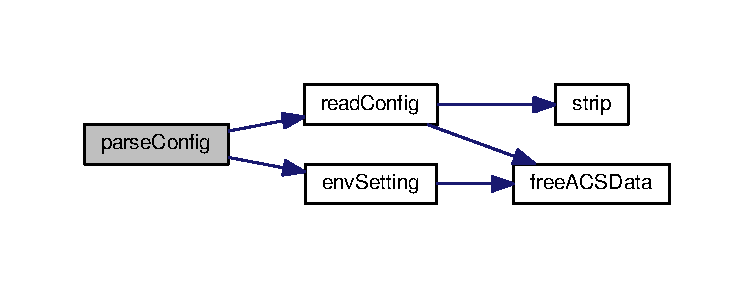
\includegraphics[width=350pt]{config_8c_a6f119b6d25f7c3bf2c8aa4770f580a95_cgraph}
\end{center}
\end{figure}


\hypertarget{config_8c_a2430ba930020227a368a1aa3bf9ef988}{\index{config.\-c@{config.\-c}!read\-Config@{read\-Config}}
\index{read\-Config@{read\-Config}!config.c@{config.\-c}}
\subsubsection[{read\-Config}]{\setlength{\rightskip}{0pt plus 5cm}static int read\-Config (
\begin{DoxyParamCaption}
\item[{char $\ast$}]{filename, }
\item[{{\bf acs} $\ast$}]{data}
\end{DoxyParamCaption}
)\hspace{0.3cm}{\ttfamily [static]}}}\label{config_8c_a2430ba930020227a368a1aa3bf9ef988}


Definition at line 151 of file config.\-c.



Here is the call graph for this function\-:\nopagebreak
\begin{figure}[H]
\begin{center}
\leavevmode
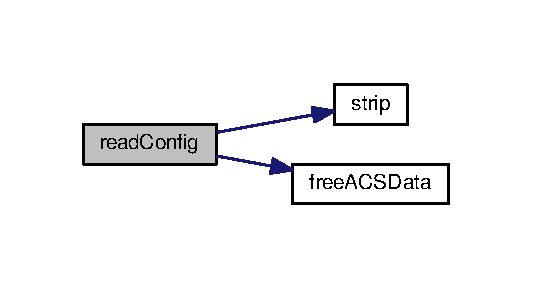
\includegraphics[width=256pt]{config_8c_a2430ba930020227a368a1aa3bf9ef988_cgraph}
\end{center}
\end{figure}


\hypertarget{config_8c_ad9a110009547c176b81af6d519486337}{\index{config.\-c@{config.\-c}!set\-A\-C\-S@{set\-A\-C\-S}}
\index{set\-A\-C\-S@{set\-A\-C\-S}!config.c@{config.\-c}}
\subsubsection[{set\-A\-C\-S}]{\setlength{\rightskip}{0pt plus 5cm}{\bf acs}$\ast$ set\-A\-C\-S (
\begin{DoxyParamCaption}
{}
\end{DoxyParamCaption}
)}}\label{config_8c_ad9a110009547c176b81af6d519486337}


Definition at line 44 of file config.\-c.

\hypertarget{config_8c_a69763ee67d1bc85f77ea1f7768a137f5}{\index{config.\-c@{config.\-c}!strip@{strip}}
\index{strip@{strip}!config.c@{config.\-c}}
\subsubsection[{strip}]{\setlength{\rightskip}{0pt plus 5cm}static void strip (
\begin{DoxyParamCaption}
\item[{char $\ast$}]{string}
\end{DoxyParamCaption}
)\hspace{0.3cm}{\ttfamily [static]}}}\label{config_8c_a69763ee67d1bc85f77ea1f7768a137f5}


Definition at line 223 of file config.\-c.



\subsection{Variable Documentation}
\hypertarget{config_8c_ad5fc7e01a4bb3aede66e4f99d8095724}{\index{config.\-c@{config.\-c}!serverdata@{serverdata}}
\index{serverdata@{serverdata}!config.c@{config.\-c}}
\subsubsection[{serverdata}]{\setlength{\rightskip}{0pt plus 5cm}{\bf acs}$\ast$ serverdata\hspace{0.3cm}{\ttfamily [static]}}}\label{config_8c_ad5fc7e01a4bb3aede66e4f99d8095724}


Definition at line 38 of file config.\-c.


\hypertarget{getdevices_8c}{\section{src/getdevices.c File Reference}
\label{getdevices_8c}\index{src/getdevices.\-c@{src/getdevices.\-c}}
}


Hold basic actions for searching, registring and deleting devices.  


{\ttfamily \#include $<$stdio.\-h$>$}\\*
{\ttfamily \#include $<$stdlib.\-h$>$}\\*
{\ttfamily \#include $<$string.\-h$>$}\\*
{\ttfamily \#include $<$ctype.\-h$>$}\\*
{\ttfamily \#include \char`\"{}ancle.\-h\char`\"{}}\\*
Include dependency graph for getdevices.\-c\-:\nopagebreak
\begin{figure}[H]
\begin{center}
\leavevmode
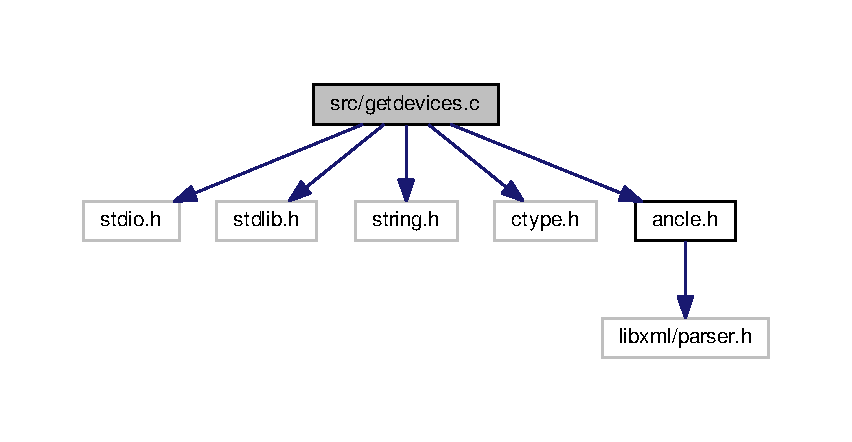
\includegraphics[width=350pt]{getdevices_8c__incl}
\end{center}
\end{figure}
\subsection*{Macros}
\begin{DoxyCompactItemize}
\item 
\#define \hyperlink{getdevices_8c_a369266c24eacffb87046522897a570d5}{\-\_\-\-G\-N\-U\-\_\-\-S\-O\-U\-R\-C\-E}
\end{DoxyCompactItemize}
\subsection*{Functions}
\begin{DoxyCompactItemize}
\item 
static \hyperlink{ancle_8h_a6a13e1aa33261886e04371dfaa52d523}{Device} $\ast$ \hyperlink{getdevices_8c_a2d6daf84c5db44bf9be326fe509bc3f6}{finddevices} (\hyperlink{ancle_8h_a6a13e1aa33261886e04371dfaa52d523}{Device} $\ast$device)
\item 
int \hyperlink{getdevices_8c_a0ea5ed437e02e57952c2302ba96adce0}{getdevices} (\hyperlink{ancle_8h_a6a13e1aa33261886e04371dfaa52d523}{Device} $\ast$device)
\begin{DoxyCompactList}\small\item\em Find devices based on parameter and display it. \end{DoxyCompactList}\item 
static int \hyperlink{getdevices_8c_a41694bbdf78727c2630dff9991b7bad0}{rm\-Device} (\hyperlink{ancle_8h_a6a13e1aa33261886e04371dfaa52d523}{Device} $\ast$device)
\item 
void \hyperlink{getdevices_8c_a6252181e611b9815d732526fabf19e0a}{rm\-Devices} (\hyperlink{ancle_8h_a6a13e1aa33261886e04371dfaa52d523}{Device} $\ast$device\-List)
\item 
int \hyperlink{getdevices_8c_afd2f9995728ed462a9e6c694a724eea8}{deldevices} (\hyperlink{ancle_8h_a6a13e1aa33261886e04371dfaa52d523}{Device} $\ast$device)
\item 
int \hyperlink{getdevices_8c_aae5f3a031a7b5db1dc464bfbeb8a4f14}{regdevice} (\hyperlink{ancle_8h_a6a13e1aa33261886e04371dfaa52d523}{Device} $\ast$device)
\end{DoxyCompactItemize}


\subsection{Detailed Description}
Hold basic actions for searching, registring and deleting devices. Functions for searching, regestring and deleteing devices wich will based on action, find desired devices on A\-C\-S server and display it on standard output or delelete it.

It will also register new device, that is defined in Device structure. 

Definition in file \hyperlink{getdevices_8c_source}{getdevices.\-c}.



\subsection{Macro Definition Documentation}
\hypertarget{getdevices_8c_a369266c24eacffb87046522897a570d5}{\index{getdevices.\-c@{getdevices.\-c}!\-\_\-\-G\-N\-U\-\_\-\-S\-O\-U\-R\-C\-E@{\-\_\-\-G\-N\-U\-\_\-\-S\-O\-U\-R\-C\-E}}
\index{\-\_\-\-G\-N\-U\-\_\-\-S\-O\-U\-R\-C\-E@{\-\_\-\-G\-N\-U\-\_\-\-S\-O\-U\-R\-C\-E}!getdevices.c@{getdevices.\-c}}
\subsubsection[{\-\_\-\-G\-N\-U\-\_\-\-S\-O\-U\-R\-C\-E}]{\setlength{\rightskip}{0pt plus 5cm}\#define \-\_\-\-G\-N\-U\-\_\-\-S\-O\-U\-R\-C\-E}}\label{getdevices_8c_a369266c24eacffb87046522897a570d5}


Definition at line 30 of file getdevices.\-c.



\subsection{Function Documentation}
\hypertarget{getdevices_8c_afd2f9995728ed462a9e6c694a724eea8}{\index{getdevices.\-c@{getdevices.\-c}!deldevices@{deldevices}}
\index{deldevices@{deldevices}!getdevices.c@{getdevices.\-c}}
\subsubsection[{deldevices}]{\setlength{\rightskip}{0pt plus 5cm}int deldevices (
\begin{DoxyParamCaption}
\item[{{\bf Device} $\ast$}]{device}
\end{DoxyParamCaption}
)}}\label{getdevices_8c_afd2f9995728ed462a9e6c694a724eea8}
Delete devices based on search paramter delete is yet not completed and will act as getdevices function 
\begin{DoxyParams}{Parameters}
{\em device} & reference device that will used as search pattern \\
\hline
\end{DoxyParams}


Definition at line 178 of file getdevices.\-c.



Here is the call graph for this function\-:\nopagebreak
\begin{figure}[H]
\begin{center}
\leavevmode
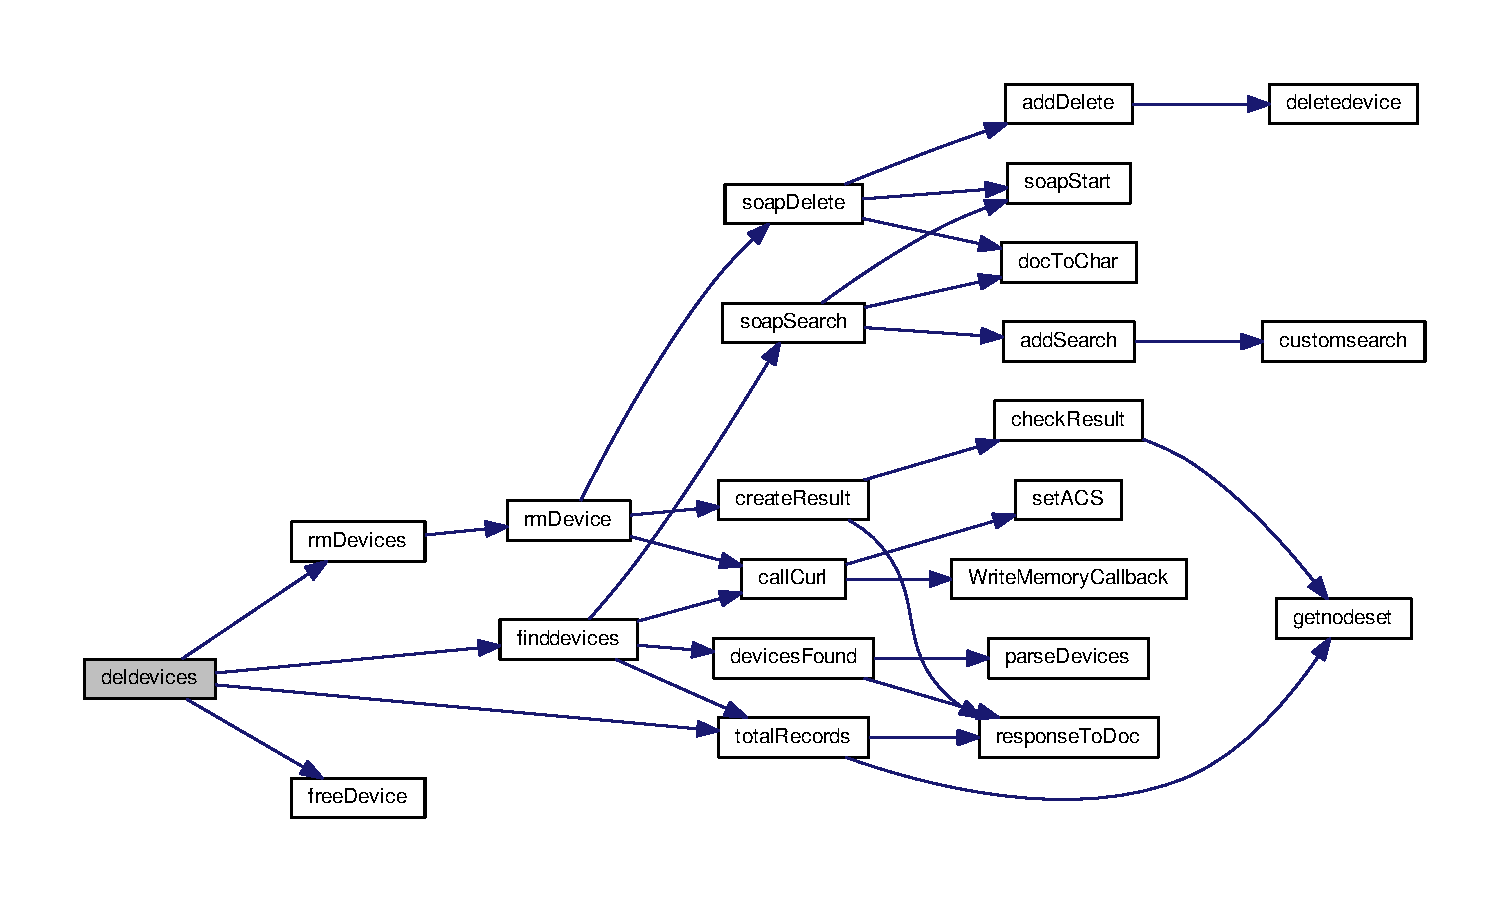
\includegraphics[width=350pt]{getdevices_8c_afd2f9995728ed462a9e6c694a724eea8_cgraph}
\end{center}
\end{figure}


\hypertarget{getdevices_8c_a2d6daf84c5db44bf9be326fe509bc3f6}{\index{getdevices.\-c@{getdevices.\-c}!finddevices@{finddevices}}
\index{finddevices@{finddevices}!getdevices.c@{getdevices.\-c}}
\subsubsection[{finddevices}]{\setlength{\rightskip}{0pt plus 5cm}static {\bf Device}$\ast$ finddevices (
\begin{DoxyParamCaption}
\item[{{\bf Device} $\ast$}]{device}
\end{DoxyParamCaption}
)\hspace{0.3cm}{\ttfamily [static]}}}\label{getdevices_8c_a2d6daf84c5db44bf9be326fe509bc3f6}
Send search request to the server and return array of devices that match criteria 
\begin{DoxyParams}{Parameters}
{\em device} & reference device that will used as search pattern \\
\hline
\end{DoxyParams}


Definition at line 45 of file getdevices.\-c.



Here is the call graph for this function\-:\nopagebreak
\begin{figure}[H]
\begin{center}
\leavevmode
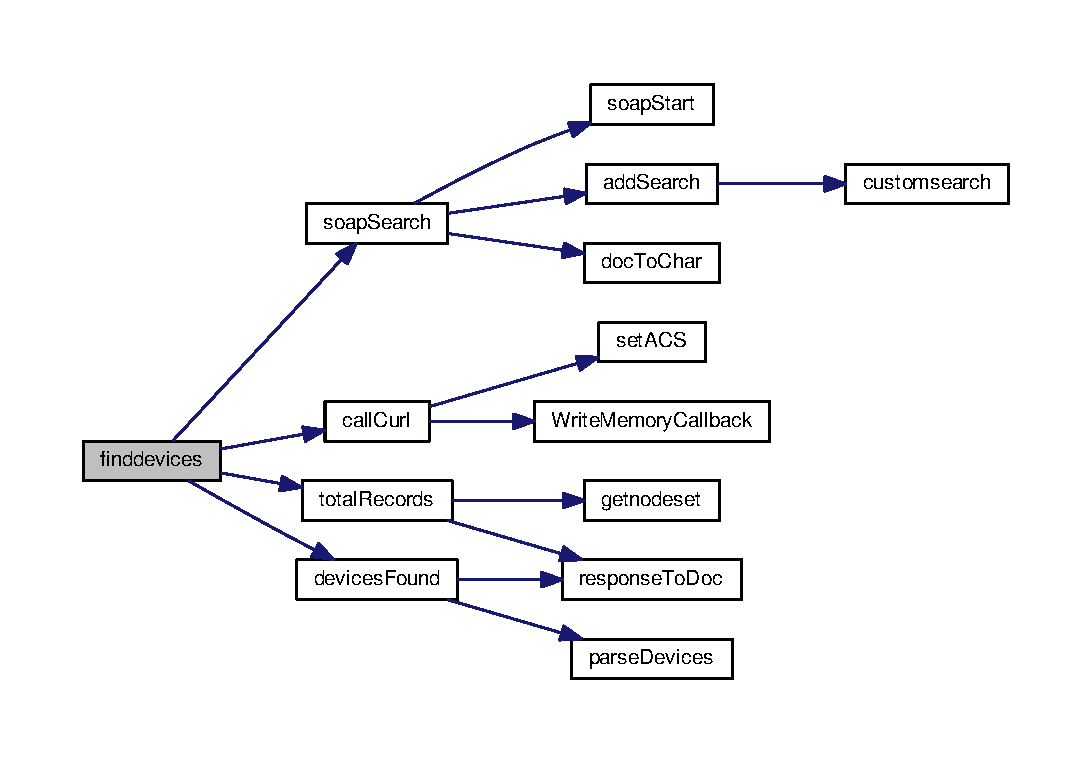
\includegraphics[width=350pt]{getdevices_8c_a2d6daf84c5db44bf9be326fe509bc3f6_cgraph}
\end{center}
\end{figure}


\hypertarget{getdevices_8c_a0ea5ed437e02e57952c2302ba96adce0}{\index{getdevices.\-c@{getdevices.\-c}!getdevices@{getdevices}}
\index{getdevices@{getdevices}!getdevices.c@{getdevices.\-c}}
\subsubsection[{getdevices}]{\setlength{\rightskip}{0pt plus 5cm}int getdevices (
\begin{DoxyParamCaption}
\item[{{\bf Device} $\ast$}]{device}
\end{DoxyParamCaption}
)}}\label{getdevices_8c_a0ea5ed437e02e57952c2302ba96adce0}


Find devices based on parameter and display it. 


\begin{DoxyParams}{Parameters}
{\em device} & reference device that will used as search pattern \\
\hline
\end{DoxyParams}


Definition at line 92 of file getdevices.\-c.



Here is the call graph for this function\-:\nopagebreak
\begin{figure}[H]
\begin{center}
\leavevmode
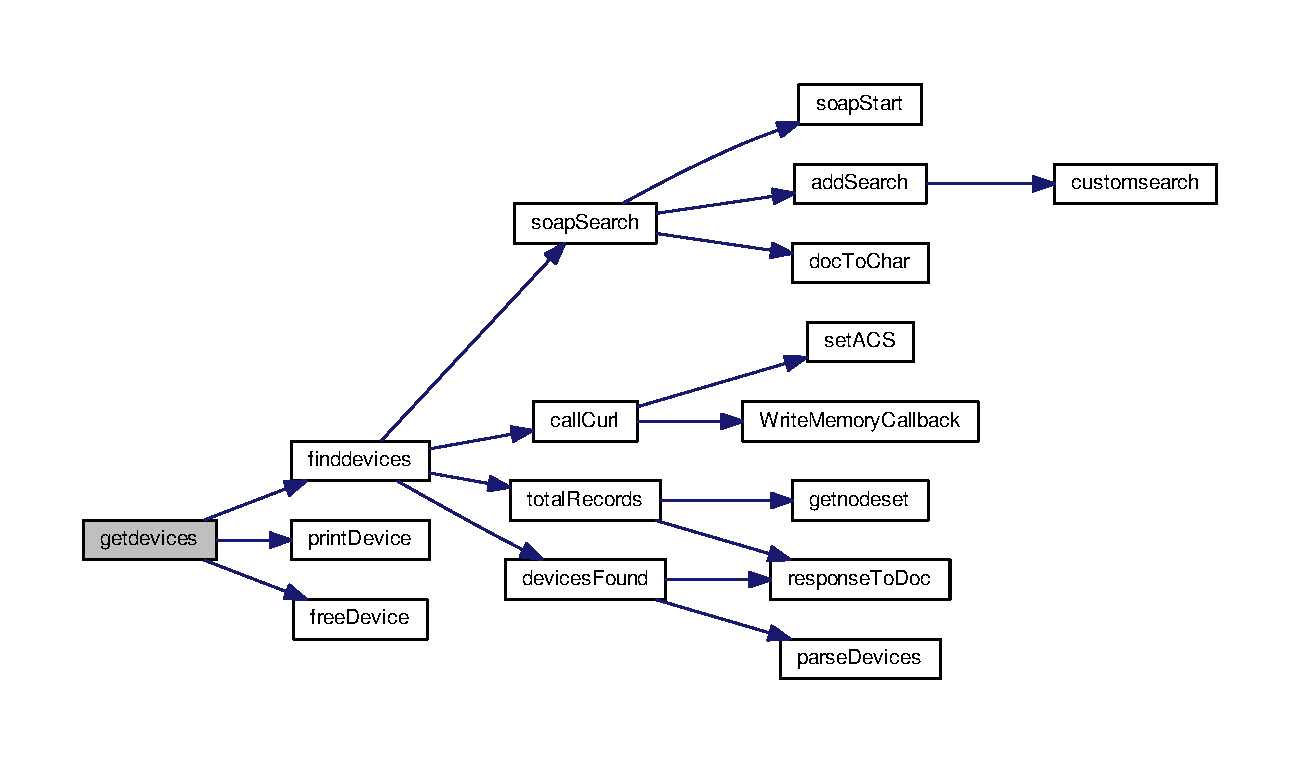
\includegraphics[width=350pt]{getdevices_8c_a0ea5ed437e02e57952c2302ba96adce0_cgraph}
\end{center}
\end{figure}


\hypertarget{getdevices_8c_aae5f3a031a7b5db1dc464bfbeb8a4f14}{\index{getdevices.\-c@{getdevices.\-c}!regdevice@{regdevice}}
\index{regdevice@{regdevice}!getdevices.c@{getdevices.\-c}}
\subsubsection[{regdevice}]{\setlength{\rightskip}{0pt plus 5cm}int regdevice (
\begin{DoxyParamCaption}
\item[{{\bf Device} $\ast$}]{device}
\end{DoxyParamCaption}
)}}\label{getdevices_8c_aae5f3a031a7b5db1dc464bfbeb8a4f14}
Used to register new device into A\-C\-S server 
\begin{DoxyParams}{Parameters}
{\em device} & must contain fully specified device \\
\hline
\end{DoxyParams}


Definition at line 213 of file getdevices.\-c.



Here is the call graph for this function\-:\nopagebreak
\begin{figure}[H]
\begin{center}
\leavevmode
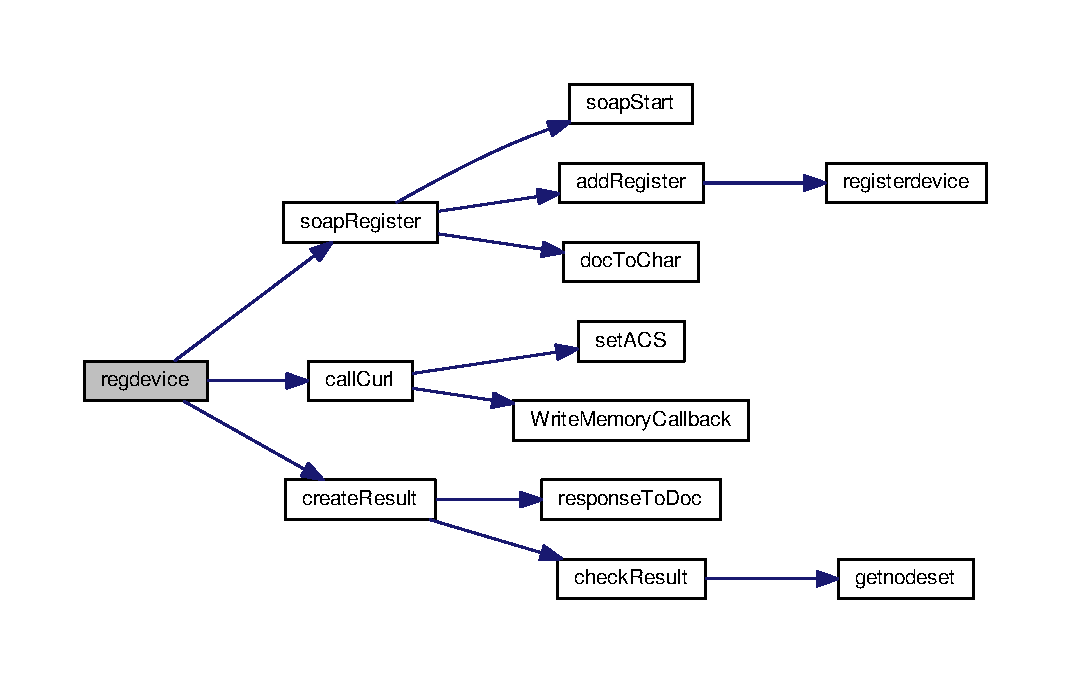
\includegraphics[width=350pt]{getdevices_8c_aae5f3a031a7b5db1dc464bfbeb8a4f14_cgraph}
\end{center}
\end{figure}


\hypertarget{getdevices_8c_a41694bbdf78727c2630dff9991b7bad0}{\index{getdevices.\-c@{getdevices.\-c}!rm\-Device@{rm\-Device}}
\index{rm\-Device@{rm\-Device}!getdevices.c@{getdevices.\-c}}
\subsubsection[{rm\-Device}]{\setlength{\rightskip}{0pt plus 5cm}static int rm\-Device (
\begin{DoxyParamCaption}
\item[{{\bf Device} $\ast$}]{device}
\end{DoxyParamCaption}
)\hspace{0.3cm}{\ttfamily [static]}}}\label{getdevices_8c_a41694bbdf78727c2630dff9991b7bad0}


Definition at line 103 of file getdevices.\-c.



Here is the call graph for this function\-:\nopagebreak
\begin{figure}[H]
\begin{center}
\leavevmode
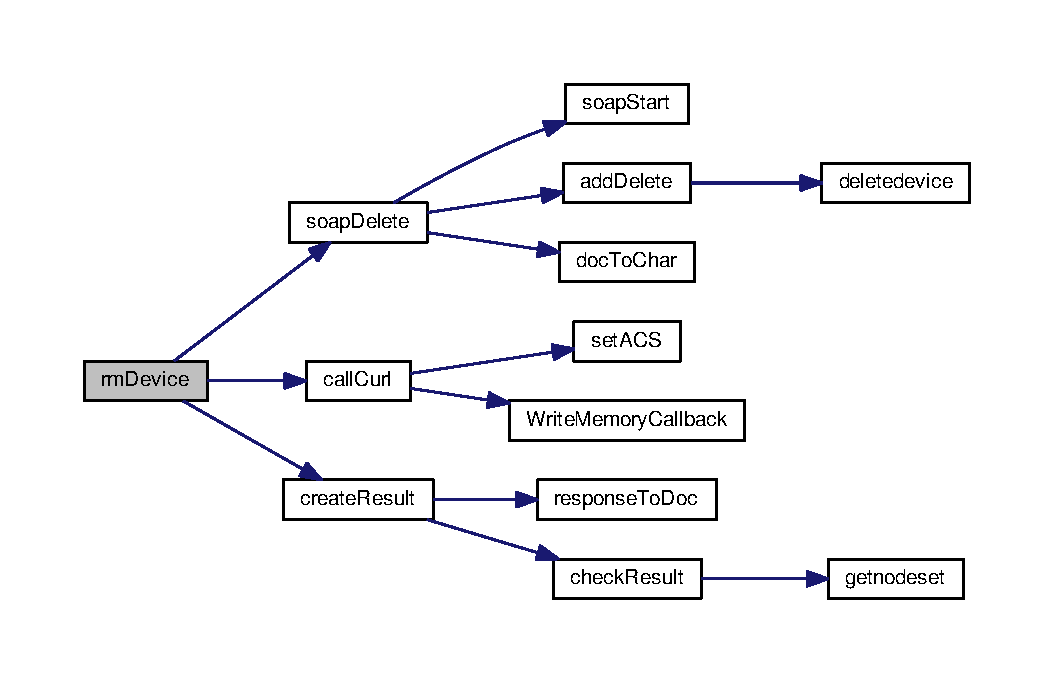
\includegraphics[width=350pt]{getdevices_8c_a41694bbdf78727c2630dff9991b7bad0_cgraph}
\end{center}
\end{figure}


\hypertarget{getdevices_8c_a6252181e611b9815d732526fabf19e0a}{\index{getdevices.\-c@{getdevices.\-c}!rm\-Devices@{rm\-Devices}}
\index{rm\-Devices@{rm\-Devices}!getdevices.c@{getdevices.\-c}}
\subsubsection[{rm\-Devices}]{\setlength{\rightskip}{0pt plus 5cm}void rm\-Devices (
\begin{DoxyParamCaption}
\item[{{\bf Device} $\ast$}]{device\-List}
\end{DoxyParamCaption}
)}}\label{getdevices_8c_a6252181e611b9815d732526fabf19e0a}
Call function to delete each individual device in the list. I will also add nubering in front of each device @ param device\-List pointer to array of devices 

Definition at line 159 of file getdevices.\-c.



Here is the call graph for this function\-:\nopagebreak
\begin{figure}[H]
\begin{center}
\leavevmode
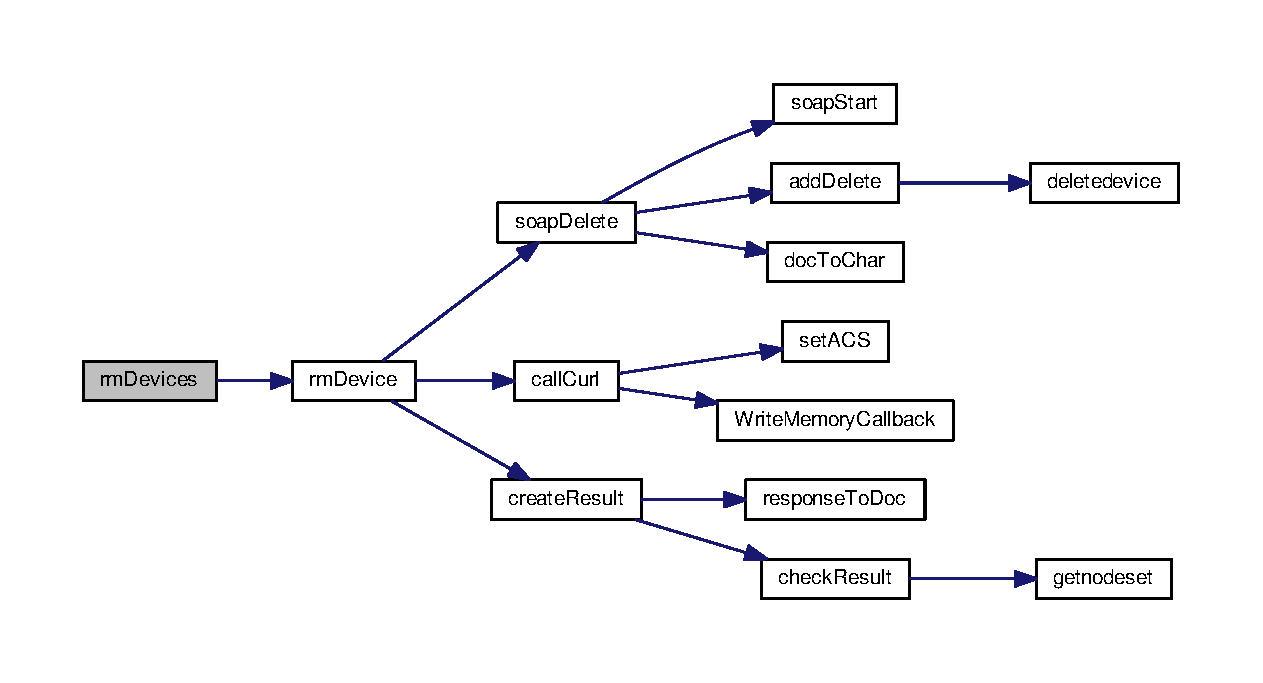
\includegraphics[width=350pt]{getdevices_8c_a6252181e611b9815d732526fabf19e0a_cgraph}
\end{center}
\end{figure}



\hypertarget{mainpage_8dox}{\section{src/mainpage.dox File Reference}
\label{mainpage_8dox}\index{src/mainpage.\-dox@{src/mainpage.\-dox}}
}

\hypertarget{parseResponse_8c}{\section{src/parse\-Response.c File Reference}
\label{parseResponse_8c}\index{src/parse\-Response.\-c@{src/parse\-Response.\-c}}
}


Functions for parsing responses from A\-C\-S server.  


{\ttfamily \#include $<$string.\-h$>$}\\*
{\ttfamily \#include $<$stdlib.\-h$>$}\\*
{\ttfamily \#include $<$libxml/parser.\-h$>$}\\*
{\ttfamily \#include $<$libxml/xpath.\-h$>$}\\*
{\ttfamily \#include \char`\"{}ancle.\-h\char`\"{}}\\*
Include dependency graph for parse\-Response.\-c\-:\nopagebreak
\begin{figure}[H]
\begin{center}
\leavevmode
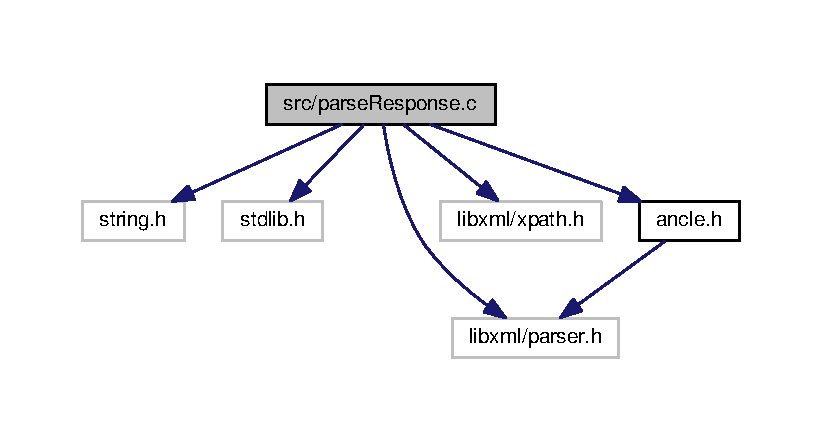
\includegraphics[width=350pt]{parseResponse_8c__incl}
\end{center}
\end{figure}
\subsection*{Macros}
\begin{DoxyCompactItemize}
\item 
\#define \hyperlink{parseResponse_8c_a150e491ed3072f46d5e7119bb2b0f50c}{name\-Ch}~(char $\ast$)name
\item 
\#define \hyperlink{parseResponse_8c_ac766be29a3aa214e6020186035034e08}{key\-Ch}~(char $\ast$)key
\end{DoxyCompactItemize}
\subsection*{Functions}
\begin{DoxyCompactItemize}
\item 
xml\-Doc\-Ptr \hyperlink{parseResponse_8c_a4bf56b0027dfa0fa5b148f2910ee077d}{response\-To\-Doc} (char $\ast$response)
\begin{DoxyCompactList}\small\item\em Create xml\-Doc from character response. \end{DoxyCompactList}\item 
static xml\-X\-Path\-Object\-Ptr \hyperlink{parseResponse_8c_aaccce875f191c49dd5b9d191a6a6b7d7}{getnodeset} (xml\-Doc\-Ptr doc, const xml\-Char $\ast$xpath)
\begin{DoxyCompactList}\small\item\em search document using xpath and return pointer \end{DoxyCompactList}\item 
void \hyperlink{parseResponse_8c_a394816653aa6d95dc72852c256d6ba5d}{free\-Device} (\hyperlink{ancle_8h_a6a13e1aa33261886e04371dfaa52d523}{Device} $\ast$device\-List)
\item 
void \hyperlink{parseResponse_8c_a7934291746b2e8dfed15ffb92af49abd}{print\-Device} (\hyperlink{ancle_8h_a6a13e1aa33261886e04371dfaa52d523}{Device} $\ast$device\-List)
\item 
int \hyperlink{parseResponse_8c_a3b80bdc3ecd85632e86c4b286a9ae0cb}{total\-Records} (char $\ast$response)
\item 
static xml\-Char $\ast$ \hyperlink{parseResponse_8c_acb703259b535250e82898c7bfc1e367d}{check\-Result} (xml\-Doc\-Ptr rsp\-Doc, const xml\-Char $\ast$xpath\-Expr)
\item 
xml\-Char $\ast$ \hyperlink{parseResponse_8c_a1c9c9a63964a0d0f06e35ce4cba3006d}{create\-Result} (char $\ast$response)
\item 
static void \hyperlink{parseResponse_8c_aac7556792151fa24981329c5fa418d7a}{parse\-Devices} (xml\-Doc $\ast$doc, xml\-Node $\ast$a\-\_\-node, \hyperlink{ancle_8h_a6a13e1aa33261886e04371dfaa52d523}{Device} $\ast$device\-List)
\begin{DoxyCompactList}\small\item\em Fill array of devices from X\-M\-L response. \end{DoxyCompactList}\item 
\hyperlink{ancle_8h_a6a13e1aa33261886e04371dfaa52d523}{Device} $\ast$ \hyperlink{parseResponse_8c_a2ff61ace0f1a1cc1f7264758b5628152}{devices\-Found} (char $\ast$response, int total)
\end{DoxyCompactItemize}


\subsection{Detailed Description}
Functions for parsing responses from A\-C\-S server. Collections of functions that will parse responses that A\-C\-S server return as answer to given request. 

Definition in file \hyperlink{parseResponse_8c_source}{parse\-Response.\-c}.



\subsection{Macro Definition Documentation}
\hypertarget{parseResponse_8c_ac766be29a3aa214e6020186035034e08}{\index{parse\-Response.\-c@{parse\-Response.\-c}!key\-Ch@{key\-Ch}}
\index{key\-Ch@{key\-Ch}!parseResponse.c@{parse\-Response.\-c}}
\subsubsection[{key\-Ch}]{\setlength{\rightskip}{0pt plus 5cm}\#define key\-Ch~(char $\ast$)key}}\label{parseResponse_8c_ac766be29a3aa214e6020186035034e08}


Definition at line 35 of file parse\-Response.\-c.

\hypertarget{parseResponse_8c_a150e491ed3072f46d5e7119bb2b0f50c}{\index{parse\-Response.\-c@{parse\-Response.\-c}!name\-Ch@{name\-Ch}}
\index{name\-Ch@{name\-Ch}!parseResponse.c@{parse\-Response.\-c}}
\subsubsection[{name\-Ch}]{\setlength{\rightskip}{0pt plus 5cm}\#define name\-Ch~(char $\ast$)name}}\label{parseResponse_8c_a150e491ed3072f46d5e7119bb2b0f50c}


Definition at line 34 of file parse\-Response.\-c.



\subsection{Function Documentation}
\hypertarget{parseResponse_8c_acb703259b535250e82898c7bfc1e367d}{\index{parse\-Response.\-c@{parse\-Response.\-c}!check\-Result@{check\-Result}}
\index{check\-Result@{check\-Result}!parseResponse.c@{parse\-Response.\-c}}
\subsubsection[{check\-Result}]{\setlength{\rightskip}{0pt plus 5cm}static xml\-Char$\ast$ check\-Result (
\begin{DoxyParamCaption}
\item[{xml\-Doc\-Ptr}]{rsp\-Doc, }
\item[{const xml\-Char $\ast$}]{xpath\-Expr}
\end{DoxyParamCaption}
)\hspace{0.3cm}{\ttfamily [static]}}}\label{parseResponse_8c_acb703259b535250e82898c7bfc1e367d}


Definition at line 124 of file parse\-Response.\-c.



Here is the call graph for this function\-:\nopagebreak
\begin{figure}[H]
\begin{center}
\leavevmode
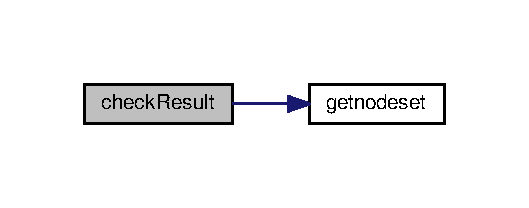
\includegraphics[width=254pt]{parseResponse_8c_acb703259b535250e82898c7bfc1e367d_cgraph}
\end{center}
\end{figure}


\hypertarget{parseResponse_8c_a1c9c9a63964a0d0f06e35ce4cba3006d}{\index{parse\-Response.\-c@{parse\-Response.\-c}!create\-Result@{create\-Result}}
\index{create\-Result@{create\-Result}!parseResponse.c@{parse\-Response.\-c}}
\subsubsection[{create\-Result}]{\setlength{\rightskip}{0pt plus 5cm}xml\-Char$\ast$ create\-Result (
\begin{DoxyParamCaption}
\item[{char $\ast$}]{response}
\end{DoxyParamCaption}
)}}\label{parseResponse_8c_a1c9c9a63964a0d0f06e35ce4cba3006d}


Definition at line 150 of file parse\-Response.\-c.



Here is the call graph for this function\-:\nopagebreak
\begin{figure}[H]
\begin{center}
\leavevmode
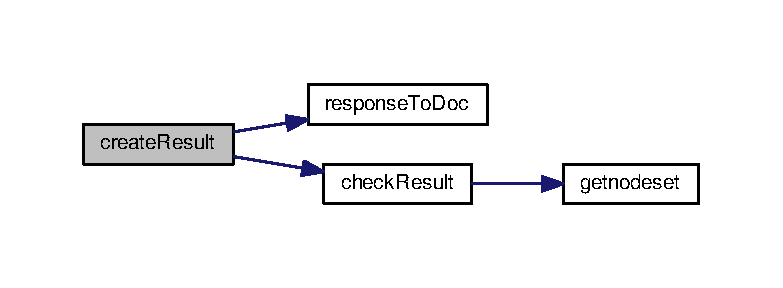
\includegraphics[width=350pt]{parseResponse_8c_a1c9c9a63964a0d0f06e35ce4cba3006d_cgraph}
\end{center}
\end{figure}


\hypertarget{parseResponse_8c_a2ff61ace0f1a1cc1f7264758b5628152}{\index{parse\-Response.\-c@{parse\-Response.\-c}!devices\-Found@{devices\-Found}}
\index{devices\-Found@{devices\-Found}!parseResponse.c@{parse\-Response.\-c}}
\subsubsection[{devices\-Found}]{\setlength{\rightskip}{0pt plus 5cm}{\bf Device}$\ast$ devices\-Found (
\begin{DoxyParamCaption}
\item[{char $\ast$}]{response, }
\item[{int}]{total}
\end{DoxyParamCaption}
)}}\label{parseResponse_8c_a2ff61ace0f1a1cc1f7264758b5628152}


Definition at line 272 of file parse\-Response.\-c.



Here is the call graph for this function\-:\nopagebreak
\begin{figure}[H]
\begin{center}
\leavevmode
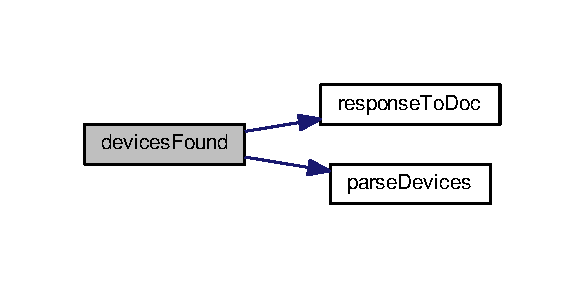
\includegraphics[width=280pt]{parseResponse_8c_a2ff61ace0f1a1cc1f7264758b5628152_cgraph}
\end{center}
\end{figure}


\hypertarget{parseResponse_8c_a394816653aa6d95dc72852c256d6ba5d}{\index{parse\-Response.\-c@{parse\-Response.\-c}!free\-Device@{free\-Device}}
\index{free\-Device@{free\-Device}!parseResponse.c@{parse\-Response.\-c}}
\subsubsection[{free\-Device}]{\setlength{\rightskip}{0pt plus 5cm}void free\-Device (
\begin{DoxyParamCaption}
\item[{{\bf Device} $\ast$}]{device\-List}
\end{DoxyParamCaption}
)}}\label{parseResponse_8c_a394816653aa6d95dc72852c256d6ba5d}


Definition at line 41 of file parse\-Response.\-c.

\hypertarget{parseResponse_8c_aaccce875f191c49dd5b9d191a6a6b7d7}{\index{parse\-Response.\-c@{parse\-Response.\-c}!getnodeset@{getnodeset}}
\index{getnodeset@{getnodeset}!parseResponse.c@{parse\-Response.\-c}}
\subsubsection[{getnodeset}]{\setlength{\rightskip}{0pt plus 5cm}static xml\-X\-Path\-Object\-Ptr getnodeset (
\begin{DoxyParamCaption}
\item[{xml\-Doc\-Ptr}]{doc, }
\item[{const xml\-Char $\ast$}]{xpath}
\end{DoxyParamCaption}
)\hspace{0.3cm}{\ttfamily [static]}}}\label{parseResponse_8c_aaccce875f191c49dd5b9d191a6a6b7d7}


search document using xpath and return pointer 


\begin{DoxyParams}{Parameters}
{\em doc} & document to search \\
\hline
{\em xpath} & search xpath expression \\
\hline
\end{DoxyParams}


Definition at line 343 of file parse\-Response.\-c.

\hypertarget{parseResponse_8c_aac7556792151fa24981329c5fa418d7a}{\index{parse\-Response.\-c@{parse\-Response.\-c}!parse\-Devices@{parse\-Devices}}
\index{parse\-Devices@{parse\-Devices}!parseResponse.c@{parse\-Response.\-c}}
\subsubsection[{parse\-Devices}]{\setlength{\rightskip}{0pt plus 5cm}static void parse\-Devices (
\begin{DoxyParamCaption}
\item[{xml\-Doc $\ast$}]{doc, }
\item[{xml\-Node $\ast$}]{a\-\_\-node, }
\item[{{\bf Device} $\ast$}]{device\-List}
\end{DoxyParamCaption}
)\hspace{0.3cm}{\ttfamily [static]}}}\label{parseResponse_8c_aac7556792151fa24981329c5fa418d7a}


Fill array of devices from X\-M\-L response. 


\begin{DoxyParams}{Parameters}
{\em doc} & X\-M\-L document \\
\hline
{\em a\-\_\-node} & starting node in X\-M\-L document  device\-List dynamic array that will be filled\\
\hline
\end{DoxyParams}
Used to parse given X\-M\-L document to fill the device list array. Function use recursion to go deep into document and pickup all device's parametes. 

Definition at line 197 of file parse\-Response.\-c.

\hypertarget{parseResponse_8c_a7934291746b2e8dfed15ffb92af49abd}{\index{parse\-Response.\-c@{parse\-Response.\-c}!print\-Device@{print\-Device}}
\index{print\-Device@{print\-Device}!parseResponse.c@{parse\-Response.\-c}}
\subsubsection[{print\-Device}]{\setlength{\rightskip}{0pt plus 5cm}void print\-Device (
\begin{DoxyParamCaption}
\item[{{\bf Device} $\ast$}]{device\-List}
\end{DoxyParamCaption}
)}}\label{parseResponse_8c_a7934291746b2e8dfed15ffb92af49abd}


Definition at line 56 of file parse\-Response.\-c.

\hypertarget{parseResponse_8c_a4bf56b0027dfa0fa5b148f2910ee077d}{\index{parse\-Response.\-c@{parse\-Response.\-c}!response\-To\-Doc@{response\-To\-Doc}}
\index{response\-To\-Doc@{response\-To\-Doc}!parseResponse.c@{parse\-Response.\-c}}
\subsubsection[{response\-To\-Doc}]{\setlength{\rightskip}{0pt plus 5cm}xml\-Doc\-Ptr response\-To\-Doc (
\begin{DoxyParamCaption}
\item[{char $\ast$}]{response}
\end{DoxyParamCaption}
)}}\label{parseResponse_8c_a4bf56b0027dfa0fa5b148f2910ee077d}


Create xml\-Doc from character response. 



Definition at line 311 of file parse\-Response.\-c.

\hypertarget{parseResponse_8c_a3b80bdc3ecd85632e86c4b286a9ae0cb}{\index{parse\-Response.\-c@{parse\-Response.\-c}!total\-Records@{total\-Records}}
\index{total\-Records@{total\-Records}!parseResponse.c@{parse\-Response.\-c}}
\subsubsection[{total\-Records}]{\setlength{\rightskip}{0pt plus 5cm}int total\-Records (
\begin{DoxyParamCaption}
\item[{char $\ast$}]{response}
\end{DoxyParamCaption}
)}}\label{parseResponse_8c_a3b80bdc3ecd85632e86c4b286a9ae0cb}
Function will parse number of devices from given S\-O\-A\-P response. If response is set to N\-U\-L\-L, then it will return last paresed, nuber of devies 

Definition at line 80 of file parse\-Response.\-c.



Here is the call graph for this function\-:\nopagebreak
\begin{figure}[H]
\begin{center}
\leavevmode
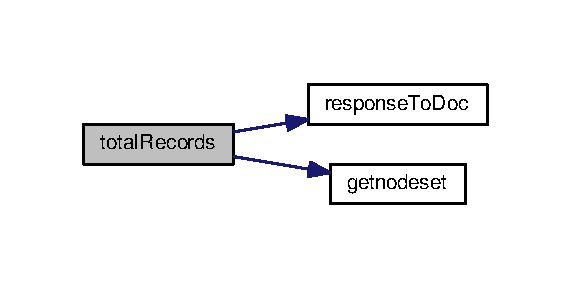
\includegraphics[width=274pt]{parseResponse_8c_a3b80bdc3ecd85632e86c4b286a9ae0cb_cgraph}
\end{center}
\end{figure}



\hypertarget{soapreq_8c}{\section{src/soapreq.c File Reference}
\label{soapreq_8c}\index{src/soapreq.\-c@{src/soapreq.\-c}}
}
{\ttfamily \#include $<$stdio.\-h$>$}\\*
{\ttfamily \#include $<$stdlib.\-h$>$}\\*
{\ttfamily \#include $<$string.\-h$>$}\\*
{\ttfamily \#include $<$libxml/parser.\-h$>$}\\*
{\ttfamily \#include $<$libxml/tree.\-h$>$}\\*
{\ttfamily \#include $<$libxml/xmlsave.\-h$>$}\\*
{\ttfamily \#include \char`\"{}ancle.\-h\char`\"{}}\\*
Include dependency graph for soapreq.\-c\-:\nopagebreak
\begin{figure}[H]
\begin{center}
\leavevmode
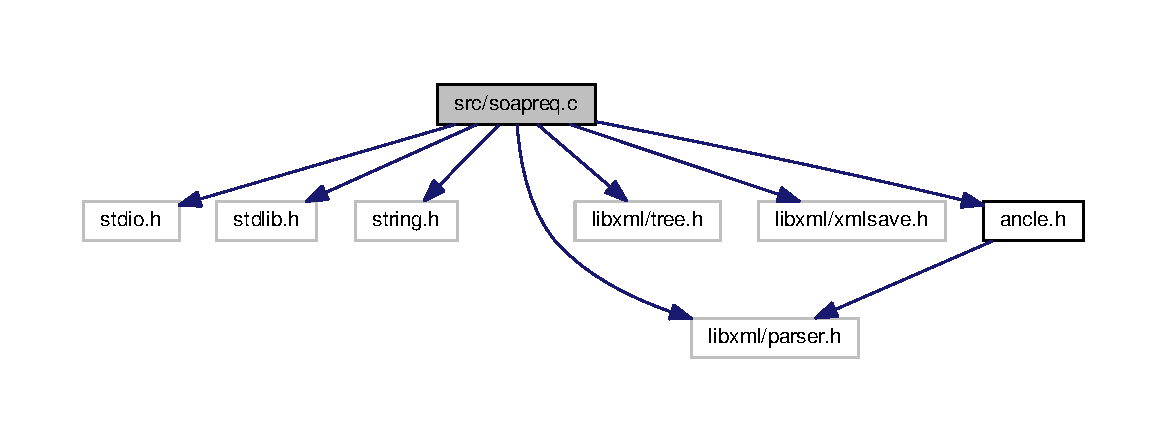
\includegraphics[width=350pt]{soapreq_8c__incl}
\end{center}
\end{figure}
\subsection*{Macros}
\begin{DoxyCompactItemize}
\item 
\#define \hyperlink{soapreq_8c_a97f6b0df98de89dd3abbb0cb8fffef3b}{D\-E\-V\-\_\-\-P\-A\-R\-A\-M\-\_\-\-S\-I\-Z\-E}~4
\end{DoxyCompactItemize}
\subsection*{Functions}
\begin{DoxyCompactItemize}
\item 
static char $\ast$ \hyperlink{soapreq_8c_acc6ae04b17e834afa30c4d8f72dadbf2}{doc\-To\-Char} (xml\-Doc\-Ptr doc)
\item 
static int \hyperlink{soapreq_8c_a8773317d857a3be3f8c8f60daa1a95d5}{registerdevice} (xml\-Node\-Ptr registerdevice, \hyperlink{ancle_8h_aead9b1579971376ebe2b29db3aacec7a}{Device\-Ptr} dev)
\item 
static int \hyperlink{soapreq_8c_a34f832bd02ca2a0702ae0c1e3d73fe05}{deletedevice} (xml\-Node\-Ptr \hyperlink{soapreq_8c_a8773317d857a3be3f8c8f60daa1a95d5}{registerdevice}, \hyperlink{ancle_8h_aead9b1579971376ebe2b29db3aacec7a}{Device\-Ptr} dev)
\item 
static int \hyperlink{soapreq_8c_a5ecb94209408af70fe0c7468f9ff3bb8}{customsearch} (xml\-Node\-Ptr customsearch, \hyperlink{ancle_8h_aead9b1579971376ebe2b29db3aacec7a}{Device\-Ptr} dev)
\item 
static xml\-Doc\-Ptr \hyperlink{soapreq_8c_a802159bda8b4e31d293a0159f530d3b5}{soap\-Start} ()
\item 
static void \hyperlink{soapreq_8c_a0b662a6ab9047c3f16c613fd17a0b7d9}{add\-Search} (xml\-Doc\-Ptr doc, \hyperlink{ancle_8h_aead9b1579971376ebe2b29db3aacec7a}{Device\-Ptr} dev)
\item 
static void \hyperlink{soapreq_8c_a645ad135c8b17c1b0b651e588344d439}{add\-Register} (xml\-Doc\-Ptr doc, \hyperlink{ancle_8h_aead9b1579971376ebe2b29db3aacec7a}{Device\-Ptr} dev)
\item 
static void \hyperlink{soapreq_8c_a11d758253f9c9eee66919446b484b538}{add\-Delete} (xml\-Doc\-Ptr doc, \hyperlink{ancle_8h_aead9b1579971376ebe2b29db3aacec7a}{Device\-Ptr} dev)
\item 
char $\ast$ \hyperlink{soapreq_8c_aa41a6f9e907badaf2f5e79a4873b100d}{soap\-Search} (\hyperlink{ancle_8h_aead9b1579971376ebe2b29db3aacec7a}{Device\-Ptr} dev)
\item 
char $\ast$ \hyperlink{soapreq_8c_ab45638d882a6836701b6afc3afa64c83}{soap\-Register} (\hyperlink{ancle_8h_aead9b1579971376ebe2b29db3aacec7a}{Device\-Ptr} dev)
\item 
char $\ast$ \hyperlink{soapreq_8c_ae4dfd1828415dc5cd6480501dc30cebb}{soap\-Delete} (\hyperlink{ancle_8h_aead9b1579971376ebe2b29db3aacec7a}{Device\-Ptr} dev)
\end{DoxyCompactItemize}


\subsection{Macro Definition Documentation}
\hypertarget{soapreq_8c_a97f6b0df98de89dd3abbb0cb8fffef3b}{\index{soapreq.\-c@{soapreq.\-c}!D\-E\-V\-\_\-\-P\-A\-R\-A\-M\-\_\-\-S\-I\-Z\-E@{D\-E\-V\-\_\-\-P\-A\-R\-A\-M\-\_\-\-S\-I\-Z\-E}}
\index{D\-E\-V\-\_\-\-P\-A\-R\-A\-M\-\_\-\-S\-I\-Z\-E@{D\-E\-V\-\_\-\-P\-A\-R\-A\-M\-\_\-\-S\-I\-Z\-E}!soapreq.c@{soapreq.\-c}}
\subsubsection[{D\-E\-V\-\_\-\-P\-A\-R\-A\-M\-\_\-\-S\-I\-Z\-E}]{\setlength{\rightskip}{0pt plus 5cm}\#define D\-E\-V\-\_\-\-P\-A\-R\-A\-M\-\_\-\-S\-I\-Z\-E~4}}\label{soapreq_8c_a97f6b0df98de89dd3abbb0cb8fffef3b}


Definition at line 28 of file soapreq.\-c.



\subsection{Function Documentation}
\hypertarget{soapreq_8c_a11d758253f9c9eee66919446b484b538}{\index{soapreq.\-c@{soapreq.\-c}!add\-Delete@{add\-Delete}}
\index{add\-Delete@{add\-Delete}!soapreq.c@{soapreq.\-c}}
\subsubsection[{add\-Delete}]{\setlength{\rightskip}{0pt plus 5cm}static void add\-Delete (
\begin{DoxyParamCaption}
\item[{xml\-Doc\-Ptr}]{doc, }
\item[{{\bf Device\-Ptr}}]{dev}
\end{DoxyParamCaption}
)\hspace{0.3cm}{\ttfamily [static]}}}\label{soapreq_8c_a11d758253f9c9eee66919446b484b538}


Definition at line 218 of file soapreq.\-c.



Here is the call graph for this function\-:\nopagebreak
\begin{figure}[H]
\begin{center}
\leavevmode
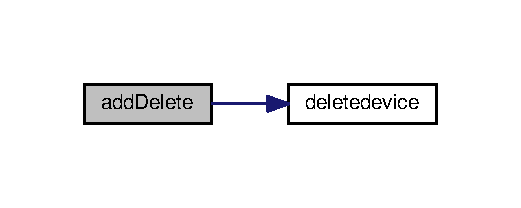
\includegraphics[width=250pt]{soapreq_8c_a11d758253f9c9eee66919446b484b538_cgraph}
\end{center}
\end{figure}


\hypertarget{soapreq_8c_a645ad135c8b17c1b0b651e588344d439}{\index{soapreq.\-c@{soapreq.\-c}!add\-Register@{add\-Register}}
\index{add\-Register@{add\-Register}!soapreq.c@{soapreq.\-c}}
\subsubsection[{add\-Register}]{\setlength{\rightskip}{0pt plus 5cm}static void add\-Register (
\begin{DoxyParamCaption}
\item[{xml\-Doc\-Ptr}]{doc, }
\item[{{\bf Device\-Ptr}}]{dev}
\end{DoxyParamCaption}
)\hspace{0.3cm}{\ttfamily [static]}}}\label{soapreq_8c_a645ad135c8b17c1b0b651e588344d439}


Definition at line 204 of file soapreq.\-c.



Here is the call graph for this function\-:\nopagebreak
\begin{figure}[H]
\begin{center}
\leavevmode
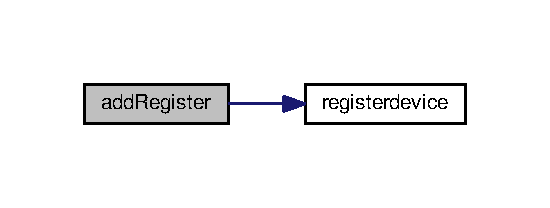
\includegraphics[width=264pt]{soapreq_8c_a645ad135c8b17c1b0b651e588344d439_cgraph}
\end{center}
\end{figure}


\hypertarget{soapreq_8c_a0b662a6ab9047c3f16c613fd17a0b7d9}{\index{soapreq.\-c@{soapreq.\-c}!add\-Search@{add\-Search}}
\index{add\-Search@{add\-Search}!soapreq.c@{soapreq.\-c}}
\subsubsection[{add\-Search}]{\setlength{\rightskip}{0pt plus 5cm}static void add\-Search (
\begin{DoxyParamCaption}
\item[{xml\-Doc\-Ptr}]{doc, }
\item[{{\bf Device\-Ptr}}]{dev}
\end{DoxyParamCaption}
)\hspace{0.3cm}{\ttfamily [static]}}}\label{soapreq_8c_a0b662a6ab9047c3f16c613fd17a0b7d9}


Definition at line 187 of file soapreq.\-c.



Here is the call graph for this function\-:\nopagebreak
\begin{figure}[H]
\begin{center}
\leavevmode
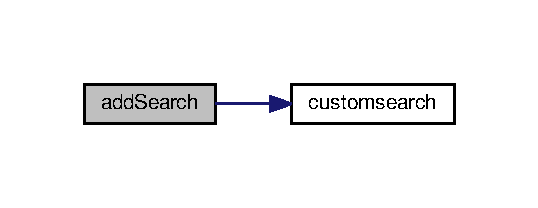
\includegraphics[width=258pt]{soapreq_8c_a0b662a6ab9047c3f16c613fd17a0b7d9_cgraph}
\end{center}
\end{figure}


\hypertarget{soapreq_8c_a5ecb94209408af70fe0c7468f9ff3bb8}{\index{soapreq.\-c@{soapreq.\-c}!customsearch@{customsearch}}
\index{customsearch@{customsearch}!soapreq.c@{soapreq.\-c}}
\subsubsection[{customsearch}]{\setlength{\rightskip}{0pt plus 5cm}static int customsearch (
\begin{DoxyParamCaption}
\item[{xml\-Node\-Ptr}]{customsearch, }
\item[{{\bf Device\-Ptr}}]{dev}
\end{DoxyParamCaption}
)\hspace{0.3cm}{\ttfamily [static]}}}\label{soapreq_8c_a5ecb94209408af70fe0c7468f9ff3bb8}


Definition at line 98 of file soapreq.\-c.

\hypertarget{soapreq_8c_a34f832bd02ca2a0702ae0c1e3d73fe05}{\index{soapreq.\-c@{soapreq.\-c}!deletedevice@{deletedevice}}
\index{deletedevice@{deletedevice}!soapreq.c@{soapreq.\-c}}
\subsubsection[{deletedevice}]{\setlength{\rightskip}{0pt plus 5cm}static int deletedevice (
\begin{DoxyParamCaption}
\item[{xml\-Node\-Ptr}]{registerdevice, }
\item[{{\bf Device\-Ptr}}]{dev}
\end{DoxyParamCaption}
)\hspace{0.3cm}{\ttfamily [static]}}}\label{soapreq_8c_a34f832bd02ca2a0702ae0c1e3d73fe05}


Definition at line 84 of file soapreq.\-c.

\hypertarget{soapreq_8c_acc6ae04b17e834afa30c4d8f72dadbf2}{\index{soapreq.\-c@{soapreq.\-c}!doc\-To\-Char@{doc\-To\-Char}}
\index{doc\-To\-Char@{doc\-To\-Char}!soapreq.c@{soapreq.\-c}}
\subsubsection[{doc\-To\-Char}]{\setlength{\rightskip}{0pt plus 5cm}static char$\ast$ doc\-To\-Char (
\begin{DoxyParamCaption}
\item[{xml\-Doc\-Ptr}]{doc}
\end{DoxyParamCaption}
)\hspace{0.3cm}{\ttfamily [static]}}}\label{soapreq_8c_acc6ae04b17e834afa30c4d8f72dadbf2}


Definition at line 31 of file soapreq.\-c.

\hypertarget{soapreq_8c_a8773317d857a3be3f8c8f60daa1a95d5}{\index{soapreq.\-c@{soapreq.\-c}!registerdevice@{registerdevice}}
\index{registerdevice@{registerdevice}!soapreq.c@{soapreq.\-c}}
\subsubsection[{registerdevice}]{\setlength{\rightskip}{0pt plus 5cm}static int registerdevice (
\begin{DoxyParamCaption}
\item[{xml\-Node\-Ptr}]{registerdevice, }
\item[{{\bf Device\-Ptr}}]{dev}
\end{DoxyParamCaption}
)\hspace{0.3cm}{\ttfamily [static]}}}\label{soapreq_8c_a8773317d857a3be3f8c8f60daa1a95d5}


Definition at line 61 of file soapreq.\-c.

\hypertarget{soapreq_8c_ae4dfd1828415dc5cd6480501dc30cebb}{\index{soapreq.\-c@{soapreq.\-c}!soap\-Delete@{soap\-Delete}}
\index{soap\-Delete@{soap\-Delete}!soapreq.c@{soapreq.\-c}}
\subsubsection[{soap\-Delete}]{\setlength{\rightskip}{0pt plus 5cm}char$\ast$ soap\-Delete (
\begin{DoxyParamCaption}
\item[{{\bf Device\-Ptr}}]{dev}
\end{DoxyParamCaption}
)}}\label{soapreq_8c_ae4dfd1828415dc5cd6480501dc30cebb}


Definition at line 250 of file soapreq.\-c.



Here is the call graph for this function\-:\nopagebreak
\begin{figure}[H]
\begin{center}
\leavevmode
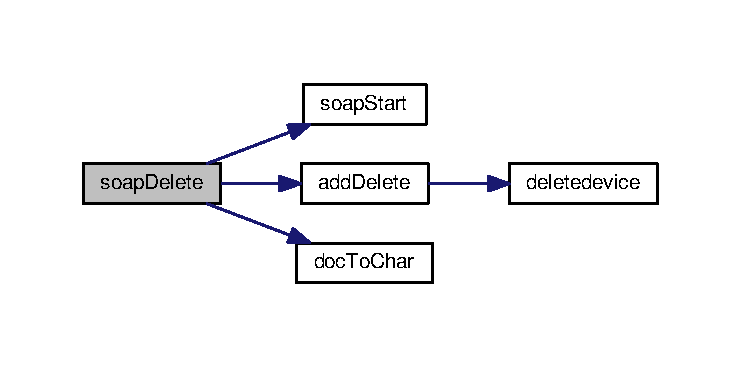
\includegraphics[width=350pt]{soapreq_8c_ae4dfd1828415dc5cd6480501dc30cebb_cgraph}
\end{center}
\end{figure}


\hypertarget{soapreq_8c_ab45638d882a6836701b6afc3afa64c83}{\index{soapreq.\-c@{soapreq.\-c}!soap\-Register@{soap\-Register}}
\index{soap\-Register@{soap\-Register}!soapreq.c@{soapreq.\-c}}
\subsubsection[{soap\-Register}]{\setlength{\rightskip}{0pt plus 5cm}char$\ast$ soap\-Register (
\begin{DoxyParamCaption}
\item[{{\bf Device\-Ptr}}]{dev}
\end{DoxyParamCaption}
)}}\label{soapreq_8c_ab45638d882a6836701b6afc3afa64c83}


Definition at line 241 of file soapreq.\-c.



Here is the call graph for this function\-:\nopagebreak
\begin{figure}[H]
\begin{center}
\leavevmode
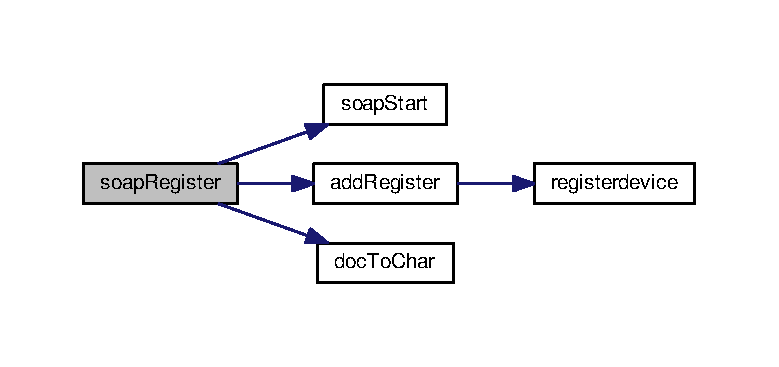
\includegraphics[width=350pt]{soapreq_8c_ab45638d882a6836701b6afc3afa64c83_cgraph}
\end{center}
\end{figure}


\hypertarget{soapreq_8c_aa41a6f9e907badaf2f5e79a4873b100d}{\index{soapreq.\-c@{soapreq.\-c}!soap\-Search@{soap\-Search}}
\index{soap\-Search@{soap\-Search}!soapreq.c@{soapreq.\-c}}
\subsubsection[{soap\-Search}]{\setlength{\rightskip}{0pt plus 5cm}char$\ast$ soap\-Search (
\begin{DoxyParamCaption}
\item[{{\bf Device\-Ptr}}]{dev}
\end{DoxyParamCaption}
)}}\label{soapreq_8c_aa41a6f9e907badaf2f5e79a4873b100d}


Definition at line 232 of file soapreq.\-c.



Here is the call graph for this function\-:\nopagebreak
\begin{figure}[H]
\begin{center}
\leavevmode
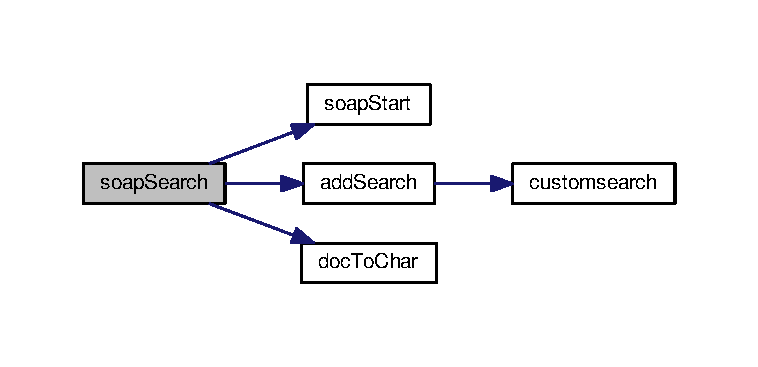
\includegraphics[width=350pt]{soapreq_8c_aa41a6f9e907badaf2f5e79a4873b100d_cgraph}
\end{center}
\end{figure}


\hypertarget{soapreq_8c_a802159bda8b4e31d293a0159f530d3b5}{\index{soapreq.\-c@{soapreq.\-c}!soap\-Start@{soap\-Start}}
\index{soap\-Start@{soap\-Start}!soapreq.c@{soapreq.\-c}}
\subsubsection[{soap\-Start}]{\setlength{\rightskip}{0pt plus 5cm}static xml\-Doc\-Ptr soap\-Start (
\begin{DoxyParamCaption}
{}
\end{DoxyParamCaption}
)\hspace{0.3cm}{\ttfamily [static]}}}\label{soapreq_8c_a802159bda8b4e31d293a0159f530d3b5}


Definition at line 164 of file soapreq.\-c.


%--- End generated contents ---

% Index
\newpage
\phantomsection
\addcontentsline{toc}{chapter}{Index}
\printindex

\end{document}
